\let\B\undefined
\newcommand{\B}{\mathcal B}
\let\T\undefined
\newcommand{\T}{\mathcal T}

\section{Sequences and Series}
[Oxford Prelims Real Analysis I]

Notes from Oxford - M1 - Sequences and Series.

\subsection{Axioms for the real numbers}
\begin{mdframed}
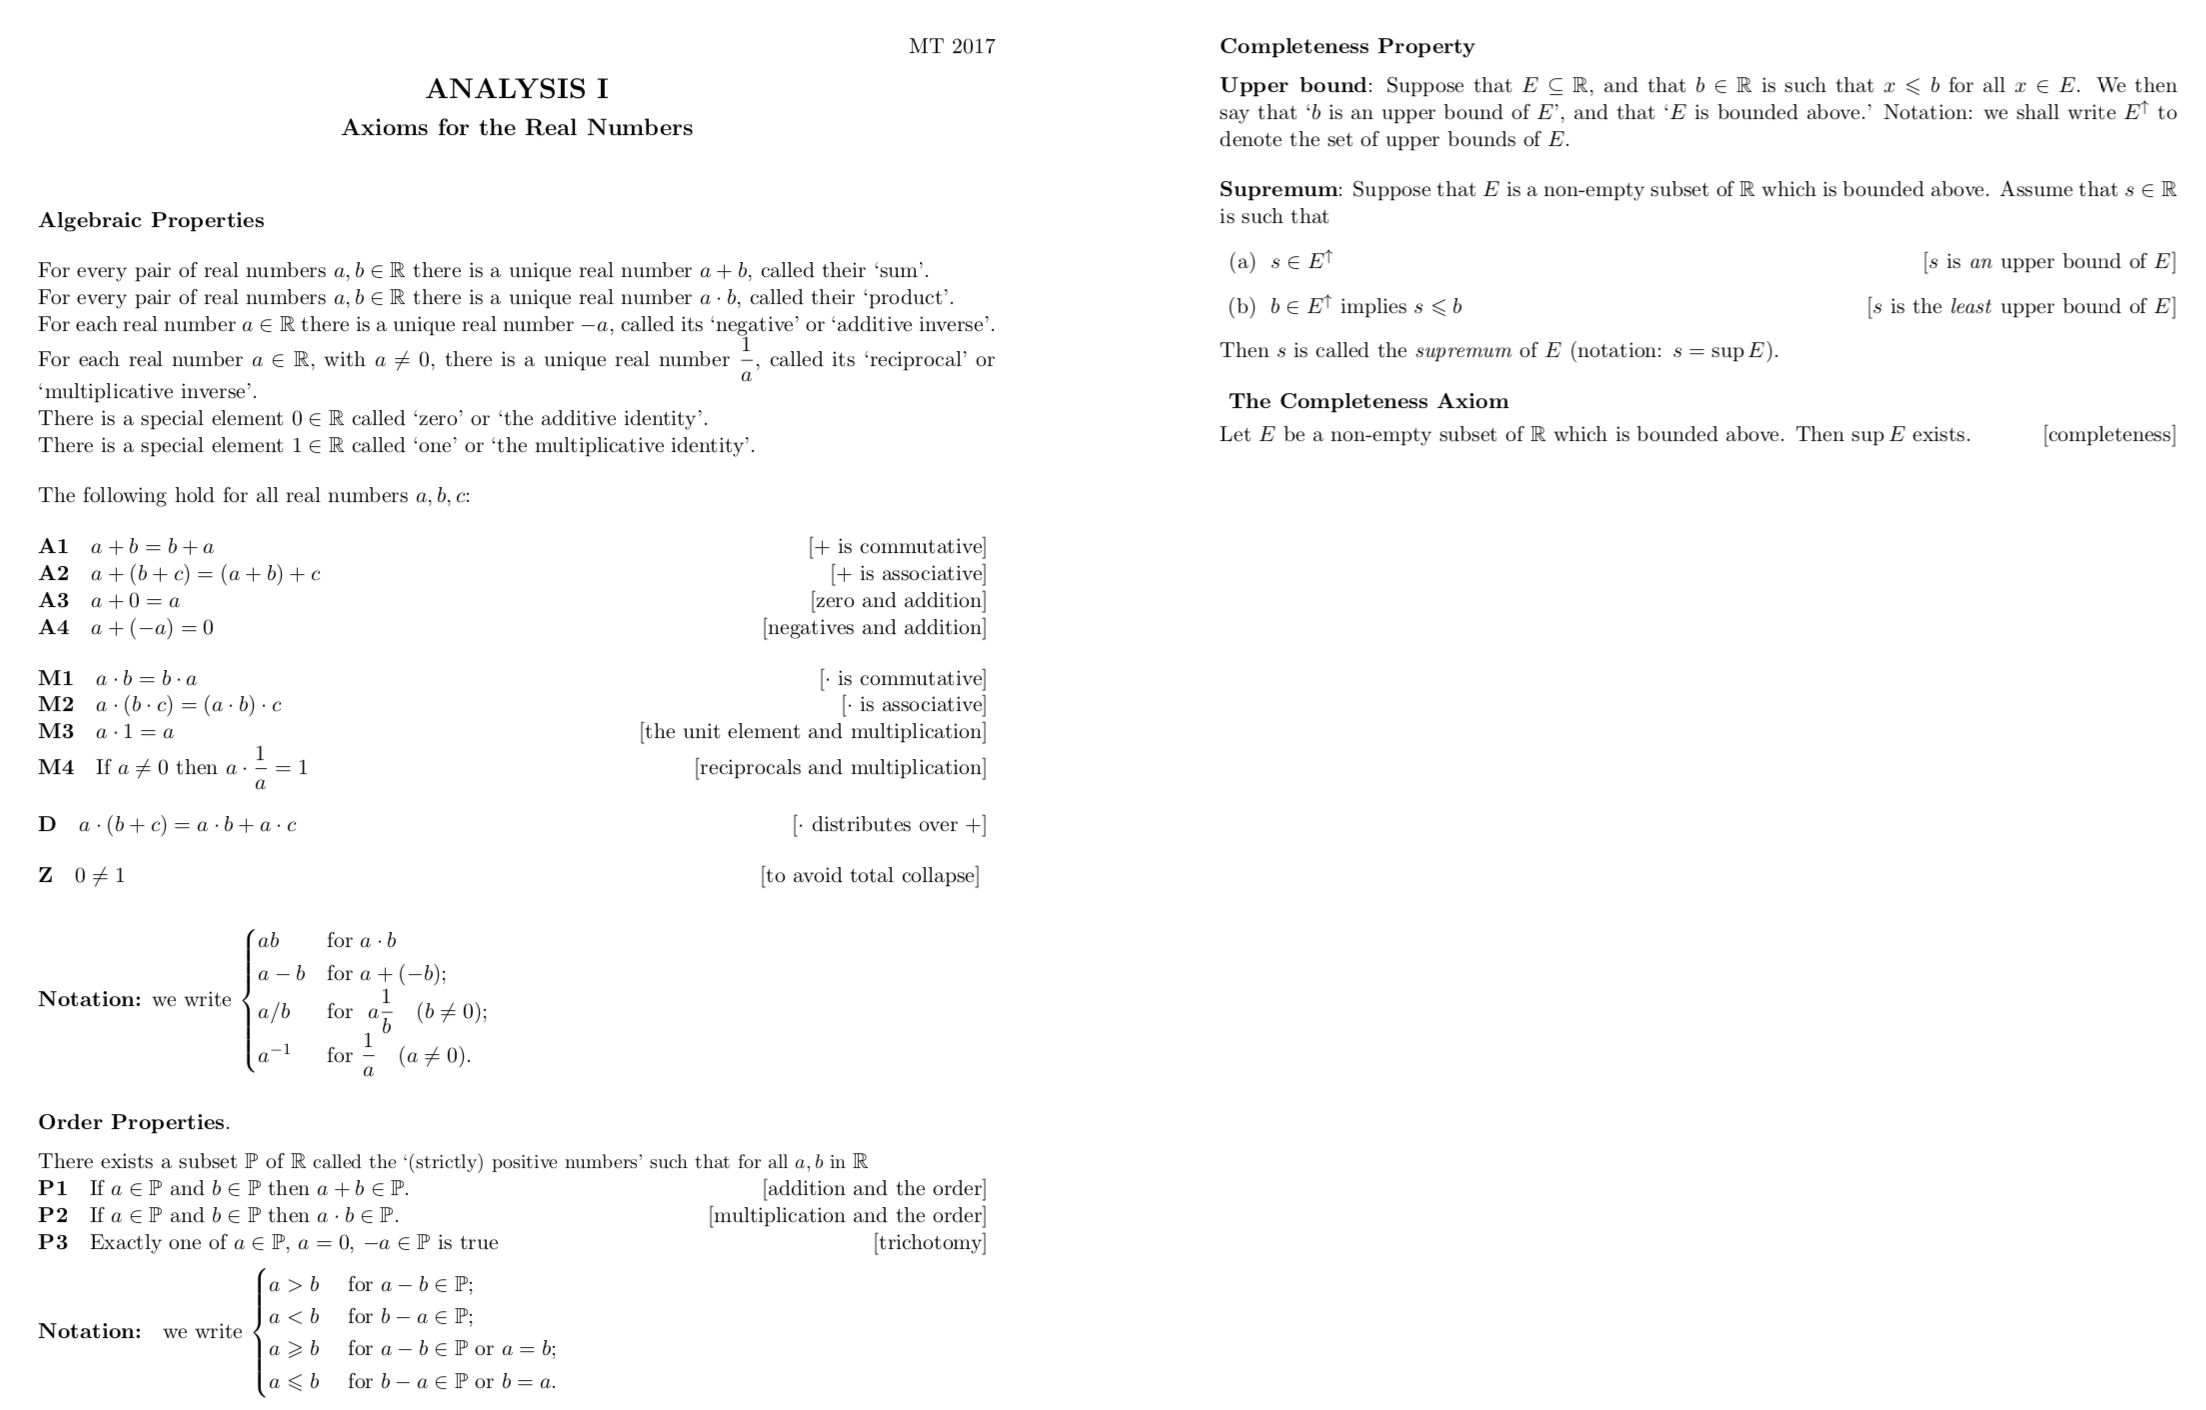
\includegraphics[width=400pt]{img/oxford-prelims-M2-analysis-I-axioms-for-real-numbers.png}
\end{mdframed}

\subsection{Approximation property of supremum}
\begin{theorem*}
  Let $S \subset \R$ be non-empty and bounded above (so $\sup S$ exists). For all $\delta > 0$,
  there exists $s_\delta \in S$ such that
  \begin{align*}
    \sup S - \delta < s_\delta \leq \sup S.
  \end{align*}
  \begin{intuition*}
    The supremum is either a member of $S$ or it is ``touching'' an element of $S$ with ``no gap''.
  \end{intuition*}
  \begin{proof}
    If $\sup S \in S$ then we can take $s_\delta = \sup S$ for all $\delta$ and we are done.

    So assume $\sup S \not\in S$. For a contradiction, suppose the negation of the claim, i.e. that
    there exists $\delta > 0$ such that for all $s \in S$ either $s \leq \sup S - \delta$ or
    $s > \sup S$. Since $s > \sup S$ is impossible by definition of $\sup$, we have that
    $s \leq \sup S - \delta$ for all $s \in S$. But then $\sup S - \delta$ is an upper bound for
    $S$ and $\sup S - \delta < \sup S$, a contradiction.
  \end{proof}
\end{theorem*}

\subsection{Archimedean Property of $\N$}
\begin{theorem*}\hspace{0pt}
  \begin{enumerate}
  \item $\N$ has no upper bound.
  \item For all $\epsilon > 0$ there exists $n \in \N$ such that $\frac{1}{n} < \epsilon$.
  \end{enumerate}
\end{theorem*}
\begin{proof}\hspace{0pt}
  \begin{enumerate}
  \item Suppose $\N$ has an upper bound. Then $\sup \N$ exists. By the Approximation Property
    there exists $n \in \N$ such that $\sup \N - \frac{1}{2} < n \leq \sup \N$. But then
    $n + 1 \in \N$ and $n + 1 > \sup N$, a contradiction. Therefore $\sup \N$ does not exist,
    therefore $\N$ has no upper bound.
  \item Since $\N$ has no upper bound, there exists $n \in \N$ such that $n > 1/\epsilon$,
    i.e. $1/n < \epsilon$.
  \end{enumerate}
\end{proof}

\subsection{Well-ordered property of $\N$}
\begin{theorem*}\hspace{0pt}
  Every nonempty subset of $\N$ has a minimum.
\end{theorem*}

\begin{proof}
  Let $\emptyset \neq S \subseteq \N \subset \R$. Note that $S$ is bounded below by 0, therefore
  $\inf S$ exists. Suppose $\inf S \not\in S$. By the Approximation Property, there exists
  $n_1 \in S$ such that $\inf S \leq n_1 < \inf S + 1$.

  We claim that $\inf S = n_1$. Suppose for a contradiction that $\inf S \neq n_1$. Then
  $n_1 = \inf S + \delta$ for some $0 < \delta < 1$. By the Approximation property again, there
  exists $n_2 \in S$ such that $\inf S \leq n_2 < n_1 < \inf S + 1$.

  But since $n_1 > n_2$ we have $n_1 \geq n_2 + 1$, therefore $n_1 \geq \inf S + 1$ which
  contradicts $n_1 < \inf S + 1$. Therefore $\inf S = n_1 \in S$ and $\min S$ exists.
\end{proof}

\begin{remark*}
  Similarly:
  \begin{enumerate}
    \item Every nonempty subset of $\Z$ that is bounded below has a minimum.
    \item Every nonempty subset of $\Z$ that is bounded above has a maximum.
  \end{enumerate}
\end{remark*}

\begin{intuition*}
  Because of the ``gappiness'' of $\N$ and $\Z$, bounded subsets must contain their suprema/infima.
\end{intuition*}

\subsection{Existence of ceil and floor}
\begin{definition*}[floor and ceil]
  Let $x \in \R$. Then floor of $x$ is $\floor{x} = \max\{n \in \Z ~|~ n \leq x\}$ and ceil of $x$
  is $\ceil{x} = \min\{n \in \Z ~|~ n \geq x\}$.
\end{definition*}

\begin{theorem*}[$\floor{x}$ and $\ceil{x}$ exist]~\\
  Let $x \in \R$. Define $S = \{n \in \Z ~|~ n \geq x\} \subset \R$. Note that $S$ is bounded below
  by $x$. Also $S$ is non-empty by the Archimedean Property of $\N$, since otherwise $x$ would be
  an upper bound for $\N$. Therefore $\ceil{x} = \min S$ exists by Well-Ordering.

  Similarly, $\floor{x}$ exists.
\end{theorem*}

\subsection{Existence of $\sqrt 2$}
\begin{theorem*}\label{existence-of-root-2}
  There exists a unique $a \in \R$ such that $a^2 = 2$.
\end{theorem*}

\begin{remark*}
  The only thing that ties the proof to the reals is that it relies on completeness ($\sup$
  exists). We know that $\sqrt 2 \not\in \Q$, therefore $\Q$ is not complete.
\end{remark*}

\begin{proof}
  Let $S = \{s \in \R ~|~ s^2 < 2\}$. Since $S$ is bounded above, $a := \sup S$ exists. We show
  that $a^2 = 2$ by showing that $a^2 < 2$ and $a^2 > 2$ lead to contradictions.

  Note that $1 \in S$, therefore $a \geq 1$.

  \begin{enumerate}
  \item {\bf Suppose $a^2 < 2$}. We seek an $h > 0$ such that $(a + h)^2 < 2$ since this would
    contradict the definition $a := \sup S$. Note that
    \begin{align*}
      (a + h)^2 - 2 &= a^2 + 2ah + h^2 - 2\\
                    &< a^2 - 2 + 3ah ~~~~~~~\text{if $h < a$}\\
                    &< 0             ~~~~~~~~~~~~~~~~~~~~~~\text{if $h < (2 - a^2)/3a$}.
    \end{align*}
    Therefore if we take $h < \min\(a, \frac{2 - a^2}{3a}\)$ then $a + h \in S$ which contradicts
    the definition $a := \sup S$.
  \item {\bf Suppose $a^2 > 2$}. By the Approximation Property for all $0 < h < 1$ we can find
    $s \in S$ such that $a - h < s$.  Therefore $(a - h)^2 < s^2 < 2$. We seek a value of $h$ such
    that $(a - h)^2 \geq 2$, which would be a contradiction. Note that $a^2 - 2ah < (a - h)^2$. If
    we take $h = (a^2 - 2)/2a$ then we have $a^2 - 2ah = 2 < (a - h)^2 < 2$, the desired
    contradiction.
  \end{enumerate}

  Finally to show that $a$ is unique, suppose that there exists $b \in \R$ with $b^2 = 2$. Then
  $0 = a^2 - b^2 = (a + b)(a - b)$ therefore $a = b$.
\end{proof}

\subsection{Connection between sequences and functions}

\begin{theorem*}
  The following two statements are equivalent:
  \begin{enumerate}
  \item $\lim_{x \to a} f(x) = L$
  \item For every sequence $(x_n)$ such that $x_n \neq a$
    \begin{align*}
      \(\lim_{n \to \infty} x_n = a\) \implies \(\lim_{n \to \infty} f(x_n) = f(a)\)
    \end{align*}
  \end{enumerate}
\end{theorem*}

\begin{intuition*}
  In other words:

  $\lim_{x \to a} f(x) = L$ if and only if the following is true:

  If $x_n \to a$ and $x_n \neq a$ then $f(x_n) \to f(a)$. I.e. $f$ is continuous.
\end{intuition*}

\begin{proof}

\end{proof}

\subsection{Limit of product is product of limits}
\red{TODO:check these proofs}
\begin{theorem*}\label{limit-of-product}~\\
  Let $\limxa f(x) = L_f$ and $\limxa g(x) = L_g$. Then
  $\limxa f(x)g(x) = L_fL_g$.
\end{theorem*}

\begin{proof}
  Note that
  \begin{align*}
    \limxa f(x)g(x) &= \limxa \Big((f(x) - L_f)(g(x) - L_g) + L_fg(x) + L_gf(x) - L_fL_g\Big)\\
                    &= L_fL_g + \limxa (f(x) - L_f)(g(x) - L_g),
  \end{align*}
  so we need to show that $\limxa (f(x) - L_f)(g(x) - L_g) = 0$. Fix $\epsilon > 0$. Since
  $\limxa (f(x) - L_f) = \limxa (g(x) - L_g) = 0$, there exists $\delta$ (pick the minimum of the
  two $\delta$s) such that whenever $|x - a| < \delta$
  \begin{align*}
    |(f(x) - L_f)| < \sqrt \epsilon ~~~\text{and}~~~|(g(x) - L_g)| < \sqrt \epsilon,
  \end{align*}
  therefore $|(f(x) - L_f)(g(x) - L_g) - 0| < \epsilon$ as required.
\end{proof}

\subsection{Limit of quotient is quotient of limits}
\red{TODO:check these proofs}
\begin{theorem*}~\\
  Let $\limxa f(x) = L_f$ and $\limxa g(x) = L_g \neq 0$. Then
  \begin{align*}
    \limxa \frac{f(x)}{g(x)} = \frac{L_f}{L_g}.
  \end{align*}
\end{theorem*}

\begin{proof}
  \red{TODO}
  \begin{align*}
    \limxa \frac{f(x)}{g(x)} - \frac{L}{M}
    = \limxa \frac{f(x)}{g(x)} - \frac{1}{g(x)} + \frac{1}{g(x)} - \frac{L}{M}
  \end{align*}

  Let $L_f = \limxa f(x)$ and $L_g = \limxa g(x) \neq 0$.

  Fix $\epsilon > 0$ and let $\delta_f$ and $\delta_g$ be such that
  \begin{align*}
    |x - a| < \delta_f \implies |f(x) - L_f| < \epsilon\\
    |x - a| < \delta_g \implies |g(x) - L_g| < \epsilon.
  \end{align*}
  Let $\delta = \min(\delta_f, \delta_g)$. Then
  \begin{align*}
    \frac{|f(x) - L_f|}{|g(x) - L_f|}
  \end{align*}
\end{proof}

\subsection{Exponential versus polynomial}
\begin{theorem*}
  $\frac{n^k}{c^n} \to 0$ as $n \to \infty$ for $k > 1$, $c > 1$.
\end{theorem*}
\begin{proof}
  Let $c = 1 + b$. Then
  \begin{align*}
    0
    < \frac{n^k}{c^n}
    &= \frac{n^k}{(1 + b)^n}\\
    &= \frac{n^k}{\sum_{i=1}^n\frac{n(n-1)\cdots(n-i+1)}{i!}b^i}\\
    &< \frac{n^k}{n(n-1)\cdots(n-k)}\frac{(k+1)!}{b^{k+1}} ~~~~~~~~\text{by retaining only the $i = k+1$ term, assuming $k+1 < n$}\\
    &< \frac{n^k}{n^{k+1}}\frac{(k+1)!}{b^{k+1}}\\
    &\to 0.
  \end{align*}
\end{proof}

\subsection{$O$ and $o$ notation}
\begin{definition*}~\\
  We write $a_n = O(b_n)$ if there exists $N \in \N$ and a constant $c > 0$ such that for all
  $n \geq N$
  \begin{align*}
    |a_n| \leq c|b_n|.
  \end{align*}
  We write $a_n = o(b_n)$ if $a_n/b_n$ is defined and $a_n/b_n \to 0$ as
  $n \to \infty$.
\end{definition*}

\begin{claim*}
  Let $a_k = \frac{(2k+1)(3k-1)}{(k+1)(k+2)^2}$. Then $a_k = O(k^{-1})$.
\end{claim*}

\begin{proof}
  \begin{align*}
    a_n &= \frac{(2n+1)(3n-1)}{(n+1)(n+2)^2}
         = \frac{6n^2 + n - 1}{n^3 + 5n^2 + 8n + 4}\\
        &=
          \frac{6}{n + 5 + 8n^{-1} + 4n^{-2}} +
          \frac{1}{n^2 + 5n + 8 + 4n^{-1}} -
          \frac{1}{n^3 + 5n^2 + 8n + 4}
  \end{align*}
\end{proof}



\subsection{Series}
\begin{definition*}~\\
  Let $(a_n)$ be a real or complex sequence.

  $s_n := \sum_{k=1}^na_k$ is the $n$th {\bf partial sum}.

  The formal summation $\sum a_n := \sum_{n=1}^\infty a_n$ is the {\bf series}\footnote{The word
    ``series'' is not always clearly defined; in particular the limit of the sum may not
    exist. Defining it as a {\it formal} (i.e. purely syntactic) summation seems to be the closest
    to a good definition.}.

  The series $\sum a_n$ converges iff $\lim_{n \to \infty} s_n$ exists.
\end{definition*}

\begin{intuition*}~\\
  The sequence $(a_n)$ is the sequence of ``steps''.

  The partial sum sequence $(s_n)$ is the sequence of locations visited.

  The series $\sum a_n$ converges if the sequence of locations converges.
\end{intuition*}

\subsection{Examples of series and power series}

\begin{tabular}{l|l|l}
  $n$th term             & Behaviour                                   & Name          \\[5pt]
  \hline&&\\
  $x^n$                  & Converges to $\frac{1}{1 - x}$ on $(-1, 1)$ & Geometric Series\\[5pt]
  $\frac{1}{n}$          & Diverges                                    & Harmonic Series \\[5pt]
  $\frac{1}{n\log n}$    & Diverges                                    &                 \\[5pt]
  $(-1)^{n+1}\frac{1}{n}$ & Converges to $\log 2$              & Alternating Harmonic Series \\[5pt]
  $\frac{x^n}{n}$        & Converges on $[-1, 1)$                      & Harmonic Series at $x=1$, Alternating Harmonic Series at $x=-1$\\[5pt]
\end{tabular}


\subsection{Series convergence theorems}

\red{These apply to complex sequences except where they involve an order relation. In that case it
  may still be useful to apply them to $|z_k|$ to establish convergence of a complex series
  $\sum z_k$ via convergence in absolute value.}

\begin{theorem*}\hspace{0pt}
  Let $a_k = s_k - s_{k-1}$ for $n \geq 2$.
  \begin{enumerate}[label=(\roman*)]
  \item $a_k \to 0$
    \begin{itemize}
    \item $\sum a_k$ converges $\implies a_k \to 0$. ({\bf Proof}: If $s_k \to L$ then $a_k = s_k - s_{k-1} \to 0$.)
    \item $a_k \to 0 \not \implies \sum a_k$ converges. ({\bf Proof}: $\sum \frac{1}{k}$, $\sum \frac{1}{k\log k}$
      do not converge)
    \end{itemize}
  \item {\bf Monotonic}: $a_k \geq 0$ and $(s_k)$ bounded above $\implies \sum a_k$ converges.
    \begin{proof}
      $\sup \{s_k\}$ exists and must be the limit.
    \end{proof}
    % \begin{proof}~\\
    %   Recall that $\sum a_k$ converges to $L$ means that for all $\epsilon > 0$ there exists
    %   $K > 0$ such that for all $k > K$ we have $|s_k - L| < \epsilon$.

    %   Let $L$ be the least upper bound for $\{s_k\}$. Fix $\epsilon > 0$.

    %   Let $K$ be such that $L - \epsilon < s_k \leq L$ (such a $K$ exists because if it did not,
    %   $L$ would not be the least upper bound).

    %   Then for all $k > K$ we have $|s_k - L| < \epsilon$.
    % \end{proof}

  \item {\bf Cauchy convergence criterion}: series converges iff sequence of partial sums is
    Cauchy. Note that $s_k - s_j = a_{j+1} + \ldots + a_k$.
  \item {\bf Comparison test; simple form}: If $0 \leq a_k \leq Cb_k$ then:
    \begin{itemize}
    \item $\sum b_k$ converges $\implies \sum a_k$ converges.
    \item Therefore also the contrapositive: $\sum a_k$ diverges $\implies \sum b_k$ diverges.
    \end{itemize}
  \item {\bf Comparison test; limit form}: If $a_k, b_k > 0$ for all $k$ and
    $\frac{a_k}{b_k} \to L$ then
    \begin{itemize}
    \item $\sum b_k$ converges $\iff \sum a_k$ converges.
    \end{itemize}
  \item {\bf Absolute convergence}:
    \begin{itemize}
    \item $\sum |a_k|$ converges $\implies$ $\sum a_k$ converges.
    \item $\sum a_k$ converges $\not \implies \sum |a_k|$ converges (alternating harmonic series
      converges to $\log 2$).
    \end{itemize}
  \item $\sum k^{-p}$ converges iff $p > 1$.
  \item {\bf Geometric series}: $\sum p^k$ series converges iff $|p| < 1$.
  \item {\bf Alternating Series Test}: $\sum (-1)^{k-1}a_k$ converges if $a_k \geq 0$ and $a_k \to 0$
    monotonically.
  \item {\bf Ratio Test}\\
    Let $L = \limk |\frac{a_{k+1}}{a_k}|$ or $L = \infty > 1$ if the limit does not exist.
    \begin{itemize}
    \item $L < 1 \implies \sum a_k$ converges.
    \item $L = 1 \implies$ inconclusive.
    \item $L > 1 \implies \sum a_k$ diverges.
    \end{itemize}
  \item {\bf Integral test}: $\sum_k f(k)$ converges iff $(I_n)$ converges, where
    $I_n = \int_1^n f(x) \dx$.
  \end{enumerate}
\end{theorem*}



\begin{remark*}
  $a_n \to 0$ does not imply that the series converges. Counterexample: the harmonic series
  $a_n = \frac{1}{n}$.
\end{remark*}

\begin{proof}\hspace{0pt}
  \begin{enumerate}[label=(\roman*)]
  \item Assume $s_n \to L$. We have $a_n = s_{n} - s_{n-1} \to L - L = 0$.
  \end{enumerate}
\end{proof}

\begin{lemma}\label{even-and-odd-subsequences-lemma}
  Let $(a_n)$ be such that $(a_{2n})$ and $(a_{2n + 1})$ both converge to $L \in \R$. Then
  $a_n \to L$.
\end{lemma}

\begin{proof}
  Fix $\epsilon > 0$. Let $N_1 \in \N$ be such that $|a_{2n} - L| < \epsilon$ for all $n \geq N_1$
  and let $N_2 \in \N$ be such that $|a_{2n + 1} - L| < \epsilon$ for all $n \geq N_2$.

  Let $N = 2\max(N_1, N_2)$. Then $|a_n - L| < \epsilon$ for all $n \geq N$, therefore $a_n \to L$.
\end{proof}

\subsection{The Harmonic Series diverges}

\begin{theorem*}
  Let $a_n = \frac{1}{n}$. Then $\sum a_n$ diverges.
\end{theorem*}

\begin{intuition*}
  In the 14th Century, Nicole d'Oresme argued that the harmonic series diverges by grouping the
  terms, after the first two, into groups of size $2, 4, 8, \ldots$.
  \begin{align*}
    \sum_{k=1}^\infty \frac{1}{k}
    &= 1 + \frac{1}{2} +
    \(\frac{1}{3} + \frac{1}{4}\) +
    \(\frac{1}{5} + \frac{1}{6} + \frac{1}{7} + \frac{1}{8}\) +
    \ldots\\
    &> 1 + \frac{1}{2} + \frac{1}{2} + \frac{1}{2} + \ldots.
  \end{align*}
  The following proof formalizes the argument.
\end{intuition*}

\begin{proof}
  Let $s_n = \sum_{k=1}^\infty a_k$. Consider
  \begin{align*}
    |s_{2^{n + 1}} - s_{2^n}|
    &= \frac{1}{2^n + 1} + \frac{1}{2^n + 2} + \ldots + \frac{1}{2^{n+1}}\\
    &\geq \frac{1}{2^{n+1}}2^n ~~~~~~~~~~~~~~\text{(smallest term) x (number of terms)}\\
    &= \frac{1}{2}.
  \end{align*}
  Therefore $(s_n)$ is not Cauchy, so $(s_n)$ diverges, i.e. $\sum a_n$ diverges.
\end{proof}

\begin{proof}
  An alternative proof uses the Integral Test. Note that $\int \frac{1}{x} \dx = \log x +
  C$. Therefore $\int_1^\infty \frac{1}{x} \dx$ does not exist (divergent). \red{incomplete}
\end{proof}


\subsection{The Alternating Series Test}
\begin{theorem}
  The series $\sum_{k\geq 1}(-1)^{k-1}a_k$ converges if
  \begin{enumerate}[label=(\roman*)]
  \item $a_k \geq 0$
  \item $a_{k+1} \leq a_k$
  \item $a_k \to 0$.
  \end{enumerate}
\end{theorem}

\begin{proof}
  \begin{intuition*}
    The steps alternate in direction and each one is smaller than the last in magnitude, so they
    always remain ``inside the previous steps''. The sequence of even-numbered locations form the
    ``lower edge'' -- a monotone increasing sequence bounded above by the first location. The proof
    demonstrates that the sequence of odd-numbered locations converges to the same location as the
    even-numbered, and therefore that the full sequence converges.
  \end{intuition*}

  Let $(s_n)$ be the sequence of partial sums. Consider the subsequence $(s_{2n})$, i.e. the
  sequence of partial sums $s_2, s_4, \ldots$. From (i) and (ii) we have
  \begin{align*}
    s_{2n}   &= a_1 - a_2 + a_3 - a_4 + \ldots + a_{2n - 1} - a_{2n}\\
             &= a_1 - (a_2 + a_3) - \ldots - (a_{2n - 2} + a_{2n - 1}) - a_{2n}\\
            &\leq a_1.
  \end{align*}
  Note that $s_{2(n+1)} - s_{2n} = a_{2n+1} - a_{2n + 2} \geq 0$, therefore $(s_{2n})$is monotone
  increasing. Also it is bounded above by $a_1$. Therefore it converges. Let $s_{2n} \to L \geq 0$.

  Note also that
  \begin{align*}
    s_{2n-1} &= s_{2n} + a_{2n} \leq a_1.
  \end{align*}
  But by (iii) we have $a_{2n} \to 0$, therefore $s_{2n-1} \to L$ also. Therefore $s_n \to L$ by lemma \ref{even-and-odd-subsequences-lemma}.
\end{proof}


\subsection{Integral Test}

\begin{intuition*}
  Basically, if $f$ is continuous and monotone decreasing for $x > N$, then
  \begin{align*}
    \int_N^\infty f(x) \dx \leq \sum_{n=N}^\infty f(n) \leq f(N) + \int_N^\infty f(x) \dx. ~~~~~~~\text{(see diagram below)}
  \end{align*}
\end{intuition*}

\begin{theorem*}[Integral Test Theorem]
  Let $f:[1,\infty] \to [0, \infty]$ be decreasing and non-negative. Define
  \begin{align*}
    s_n = \sum_{k=1}^nf(k) ~~~~~~~~~~~~~ I_n = \int_1^n f(x) \dx ~~~~~~~~~~~~~ \sigma_n = s_n - I_n.
  \end{align*}
  Then $\sigma_n \to \sigma$, where $0 \leq \sigma \leq f(1)$.
\end{theorem*}

\begin{corollary*}[Integral Test]
  $(s_n)$ converges if and only if $(I_n)$ converges.
\end{corollary*}

\begin{intuition*}\hspace{0pt}
  \begin{mdframed}
    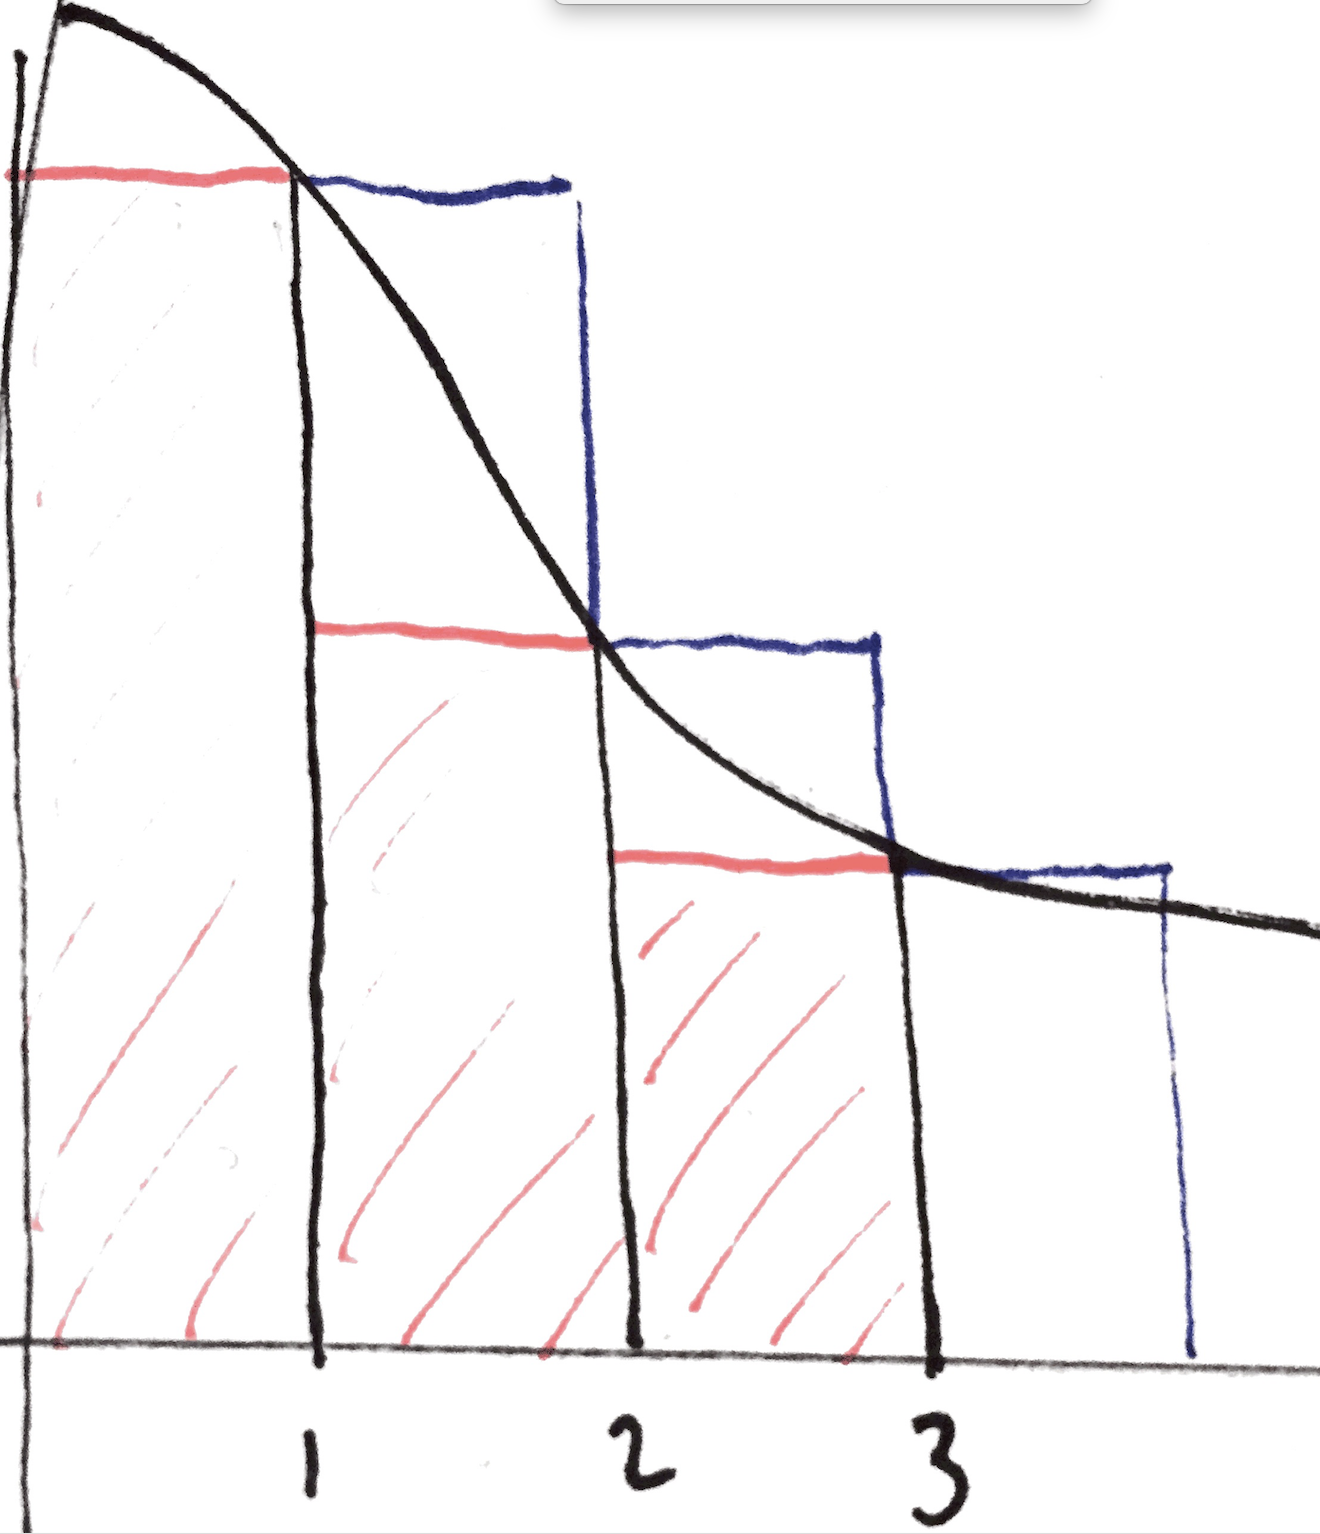
\includegraphics[width=200pt]{img/analysis--integral-test-theorem.png}

    The combined area of the 3 blue rectangles ($s_3 = f(1) + f(2) + f(3)$) exceeds the area
    $\int_1^3 f(x) \dx$. But the difference is less than $f(1)$. I.e.
    \begin{align*}
      f(1) + f(2) + f(3) \leq f(1) + \int_1^3 f(x) \dx
    \end{align*}


  \end{mdframed}
\end{intuition*}

\begin{proof}
  See notes.
\end{proof}



\subsection{Abel's theorem}
\begin{theorem*}
  Let $\sum_{n=0}^\infty a_nx^n$ be a power series with real coefficients $a_n$, convergent on
  $(-1, 1)$. Then $f$ given by $f(x) = \sum_{n=0}^\infty a_nx^n$ is left-continuous at $x=1$.
\end{theorem*}

\subsection{Alternating harmonic series}
\begin{theorem*}
  $\sum_{n=1}^\infty (-1)^{n+1}\frac{1}{n} = \log 2$.
\end{theorem*}

\begin{proof}

\end{proof}

Note that for $-1 < x < 1$ the series $\sum_{n=0}^\infty (-x)^n$ converges to
$\frac{1}{1+x}$. Therefore, using the term-by-term integration theorem for power series,
\begin{align*}
  \int\(\sum_{n=0}^\infty (-x)^n\) \dx
  = \sum_{n=0}^\infty \frac{(-x)^{n+1}}{n+1}
  = \sum_{n=1}^\infty \frac{(-x)^n}{n}
  = C + \log(1 + x),
\end{align*}
and taking $x=0$ shows that $C = 0$.

\begin{remark*}\hspace{0pt}
  \begin{enumerate}
  \item If it were valid to plug in $x=-1$ we would have the desired result
    $\sum_{n=1}^\infty \frac{(-1)^{n+1}}{n} = \log(2)$. However, this is not a proof, since the
    above argument is based on a geometric series with an interval of convergence of $-1 < x < 1$.
  \item The series $\sum_{n=1}^\infty \frac{(-1)^{n+1}}{n}$ does converge, by the Alternating
    Series Test. (The AST does not tell us what that limit is.)
  \end{enumerate}
\end{remark*}

Let $f$ be given by $f(x) = \sum_{n=1}^\infty \frac{(-x)^{n}}{n} = \log(1 + x)$. By Abel's theorem,
$f$ is continuous at the boundary point $x = 1$. I.e.
\begin{align*}
  \lim_{x\uparrow 1} \sum_{n=1}^\infty \frac{x^n}{n} = \log(2).
\end{align*}




\subsection{Power series}

\begin{definition*}
  A complex power series is a series of the form $\sum c_kz^k$, where $c_k, z \in \C$.

  The series defines a function with domain equal to the region of convergence and codomain $\C$.

  If $c_k, z \in \R$ then it is a real power series.
\end{definition*}

\begin{example*}
  We {\bf define}
  \begin{align*}
    e^z     &= \sum_{k=0}^\infty \frac{1}{k!}z^k\\
    \\
              \sin z  &= \sum_{k=0}^\infty (-1)^k\frac{1}{(2k+1)!}z^{2k + 1}\\
    \cos z  &= \sum_{k=0}^\infty (-1)^k\frac{1}{(2k)!}z^{2k}\\
    \\
    \sinh z &= \sum_{k=0}^\infty \frac{1}{(2k+1)!}z^{2k + 1}\\
    \cosh z &= \sum_{k=0}^\infty \frac{1}{(2k)!}z^{2k}
  \end{align*}
  In all cases the Ratio Test proves convergence in absolute value for all $z \in \C$.

  Identities:
  \begin{align*}
    \cos z  &= \frac{1}{2}(...)\\
    \cosh z &= \frac{1}{2}(...)\\
    \sin z  &= \frac{1}{2}(...)\\
    \sinh z &= \frac{1}{2}(...)\\
    e^{iz} &= ...
  \end{align*}
\end{example*}

\begin{definition*}
  The radius of convergence is
  \begin{align*}
    R =
    \begin{cases}
      \sup \Big\{|z| ~\Big|~ \sum|c_kz^k| ~\textup{converges}\Big\}, &\textup{if the supremum exists}\\
      \infty, &\textup{otherwise}.
    \end{cases}
  \end{align*}
\end{definition*}

\begin{remark*}
  So the radius of convergence is (informally) the furthest distance from the origin at which the
  series still converges. One might think that the set of values $z$ where the series converges
  would not define a region with a simple shape. However, the next theorem shows that the region is
  in fact a disc:
\end{remark*}

\begin{theorem*}
  Let $\sum c_kz^k$ be a power series with radius of convergence $R > 0$. Then
  \begin{enumerate}
  \item $\sum |c_kz^k|$ converges for all $|z| < R$, and hence $\sum c_kz^k$ converges.
  \item $\sum c_kz^k$ diverges for $|z| > R$.
  \end{enumerate}
  At $|z| = R$ it may converge or diverge.
\end{theorem*}

\begin{proof}~\\~\\
  {\bf Informal proof of (1):} The key here is
  \begin{enumerate}
  \item convergence in absolute value implies convergence, and
  \item the Comparison Test (Simple Form), which is used to show that a series of smaller absolute
    values converges if a series of larger absolute values does.
  \end{enumerate}
  The theorem is fairly obvious for a real power series: if the radius of convergence is $R$ then
  the series must converge at a value arbitrarily close to either $-R$ or $R$. Call this value
  $x$. So $\sum |c_kx^k| = \sum |c_k||x_k|$ converges. Now consider some other value $t$ with
  $|t| < |x|$. We have that $\sum |c_kt_k|$ converges by the Comparison Test (Simple Form) and
  hence $\sum c_kt_k$ converges.

  The thing is that this works similarly for a complex power series, since convergence in absolute
  value implies convergence for complex series also:

  Fix $R > 0$ and consider the circle with radius $R$ centered on the origin. Fix $z \in \C$ such
  that $|z| < R$. Note that there must be some $\rho \in \C$ such that $|z| < |\rho| \leq R$ and
  $\sum |c_k\rho^k|$ converges, otherwise $R$ would not be the supremum. But
  $|c_kz^k| < |c_k\rho^k|$ for all $k$ and so $\sum |c_kz^k|$ converges by the Comparison Test
  (Simple Form), and hence $\sum c_kz^k$ converges.

  {\bf Informal proof of (2):} Fix $z$ such that $|z| > R$.

  (Then $\sum |c_kz^k|$ does not converge, since otherwise $R$ would not be the supremum. But lack
  of convergence in absolute value doesn't prove divergence: e.g. the alternating harmonic series
  converges.)

  \red{TODO}

\end{proof}


\section{Continuity and Differentiability}
[Oxford Prelims Real Analysis II]

Notes from Oxford - M2 - Continuity and Differentiability.

\subsection{Limit point}
\begin{definition*}
Let $E \subset \R$. A point $p \in \R$ is a limit point of $E$ iff for all $\delta > 0$ there
exists $x \in E$ such that $0 < |x - p| < \delta$.
\end{definition*}
\begin{intuition*}
  A deleted ball (segment), of arbitrarily small radius (length), placed over $p$, will capture at
  least one point of $E$.
\end{intuition*}

\subsection{Limit, Convergence}

\begin{definition*}[Limit of a sequence $(x_n)$]~\\
  $\lim_{n \to \infty} x_n = L$ iff for all $\epsilon > 0$ there exists $N \in \N$ such that
  $n > N \implies |x_n - L| < \epsilon$. The sequence is then said to \textit{converge} to $L$.
\end{definition*}

\begin{definition*}[Limit of a function $f:\R\to\R$]~\\
  $\lim_{x \to a} f(x) = L$ means: for all $\epsilon > 0$ there exists $\delta > 0$ such that
  $0 < |x - a| < \delta \implies |f(x) - L| < \epsilon$.
\end{definition*}

Equivalent notation: $f(x) \to L$ as $x \to a$

\begin{remark*}\hspace{0pt}
  \begin{enumerate}
  \item The value of $f$ at $a$ is irrelevant ($f$ need not be defined at $a$).
  \item $f$ must tend to $L$ from both sides.
  \end{enumerate}
\end{remark*}

\subsection{Limits involving $\infty$}

\begin{definition*}
  $\lim_{n \to \infty} x_n = \infty$ if for all $X \in \R$ there exists $N \in \N$ such that
  $n \geq N \implies x_n > X$.
\end{definition*}

\begin{definition*}
  $\lim_{x \to \infty} f(x) = L$ if for all $\epsilon > 0$ there exists $X \in \R$ such that
  $x > X \implies |f(x) - L| < \epsilon$.
\end{definition*}

\begin{theorem*}[I assume. Have not proved this.]
  $\lim_{x \to \infty} f(x) = L$ iff for all sequences $(x_n)$ such that
  $\lim_{n \to \infty}x_n = \infty$ we have $\lim_{n \to \infty} f(x_n) = L$.
\end{theorem*}

\subsection{Limits of functions - Examples}

\begin{example}
  Let $E = \R\setminus \{0\}$ and define $f:E \to \R$ by $f(x) = L$. Then 0 is a limit point of
  $E$ and $f(x) \to L$ as $x \to 0$.
\end{example}

\begin{proof}
  Fix $\delta > 0$. Then $\exists x ~ 0 < |x - 0| < \delta$ is true since we can choose
  $x = \frac{\delta}{2}$. Therefore 0 is a limit point of $E$.

  Fix $\epsilon > 0$. Let $\delta = 1$. Then
  $0 < |x - 0| < \delta \implies |f(x) - L| = 0 < \epsilon$.
\end{proof}

\subsection{Continuity of a function $f$}

\begin{definition*}
$f$ is continuous at $a$ if $\lim_{x \to a} f(x) = f(a)$.
\end{definition*}

Therefore, using the definition of limit, $f$ is continuous at $a$ iff for all $\epsilon > 0$
there exists $\delta > 0$ such that $|x - a| < \delta \implies |f(x) - f(a)| < \epsilon$.

\subsection{Uniform convergence and uniform continuity}

\begin{definition*}[Uniform convergence]
A sequence of functions $\{f_n\}_{n\geq 0}$ has a limit $f$ iff for every point
$x$ in the input set the sequence $\{f_n(x)\}_{n\geq 0}$ has limit $f(x)$.

They \textit{converge uniformly} to $f$ iff the same $m$ works for all input
values.
\end{definition*}

\begin{definition*}[Uniform continuity]
A function $f$ is uniformly continuous iff the same $\delta$ works for all $x_0$.

A function $f$ is uniformly continuous iff for all $\epsilon$, no matter how
small, a $\delta$ exists such that for all $x_0 \in U$, if $x$ is within
$\delta$ of $x_0$ then $f(x)$ is within $\epsilon$ of $f(x_0)$.
\end{definition*}

\subsection{Intermediate value theorem}
\begin{theorem*}
  Let $a, b \in \R$ with $b > a$, and $f:[a,b] \to \R$ be continuous. Let $u$ lie strictly between
  $f(a)$ and $f(b)$. Then there exists $c \in (a, b)$ such that $f(c) = u$.
\end{theorem*}

\begin{proof}
  Define $S := \{x \in [a, b] ~|~ f(x) < u\}$. Since $a \in S$, $S$ is non-empty. By completeness
  of reals $c := \sup S$ exists. The theorem now follows from continuity of $f$ at $c$. (Fix
  $\epsilon > 0$ and consider points $a^* \in (c - \delta, c)$ and $a^{**} \in (c, c + \delta)$,
  noting whether they are in $S$ and the $\epsilon-\delta$ continuity criterion.)
\end{proof}


\subsection{Mean-value theorem}
\begin{theorem*}
  Let $a, b \in \R$ with $b > a$, and $f:[a,b] \to \R$ be continuous on $[a, b]$ and differentiable
  on $(a, b)$. Then there exists $x \in (a, b)$ such that $f'(x) = \frac{f(b) - f(a)}{(b - a)}$.
\end{theorem*}


\subsection{Differentiability implies continuity}
\begin{theorem*}
  Let $f:\R\to\R$ be differentiable. Then $f$ is continuous.
\end{theorem*}

\begin{proof}~\\
  Let $a \in \R$. The claim is that $\limxa f(x) - f(a) = 0$. Since $f$ is differentiable,
  \begin{align*}
    f'(a) &= \lim_{x \to a} \frac{f(x) - f(a)}{x - a}
  \end{align*}
  exists. Therefore by \eqref{limit-of-product}
  \begin{align*}
    \lim_{x \to a} f(x) - f(a) = \lim_{x \to a} (x - a)\frac{f(x) - f(a)}{x - a} = 0\cdot f'(a) = 0.
  \end{align*}
\end{proof}

\begin{remark*}
  Intuitively it seems that differentiability implies continuity because, for the derivative to
  exist, the numerator $f(x) - f(a)$ must get small as $x\to a$, as the denominator $x - a$ does.
\end{remark*}


\newpage
\section{Integration}
[Oxford Prelims Real Analysis III]
\red{(not studied)}

The Riemann integral of the indicator function of the rationals? $\int_0^1 {\bf 1}_\Q$ is undefined.

This is because any open interval contains both rational and irrational points, hence the majorant (supremum
approximation) would be $\geq 1$ and the minorant (infimum approximation) would be $\leq 0$ and they can never
agree.

\section{Metric Spaces}
[Oxford Part A 2]

\subsection{Distance metrics and norms}

\begin{enumerate}
\item A \defn{metric space} is a set of objects with a \defn{distance metric}.
\item A distance metric is a function that assigns a non-negative real number to every pair of
  elements.
\item Note that addition is not necessarily defined on the metric space but is, of course, defined
  on the distances.
\item Some metric spaces are \defn{vector spaces}. In a vector space, addition is defined and there
  is an additive identity (the ``origin'').
\item Some vector spaces possess a \defn{norm}. A norm $\|.\|$ is a function that assigns a
  non-negative real number to every vector.
\item If a vector space has a norm, this gives a natural distance metric: $d(x, y) = \|x -
  y\|$. Therefore we can think of the norm of a vector as its distance from the origin.
\item Some vector spaces possess an \defn{inner product}.
\item If a vector space has a {\it real} inner product, this gives a natural norm:
  $\|u\| = \< u, u\>$, and thus a natural distance metric:
  $d(x, y) = \|x - y\| = \< x - y, x - y \>$.
\item Requirements

  % #+ORGTBL: SEND metric-norm-inner-product orgtbl-to-latex :splice nil :skip 0 :raw t
  % |                       | distance metric                  | norm                                    | real inner product                              |
  % |-----------------------+----------------------------------+-----------------------------------------+-------------------------------------------------|
  % | positive definiteness | $d(x, y) = 0 \iff x = y$         | $\norm{u} = 0 \iff u = 0$               | $\< v, v\> = 0 \iff v = 0$                      |
  % | triangle inequality   | $d(x, z) \leq d(x, y) + d(y, z)$ | $\norm{u + v} \leq \norm{u} + \norm{v}$ | definition $\implies$ C-S $\implies$ tri. ineq. |
  % | symmetry              | $d(x, y) = d(y, x)$              | N/A                                     | $\< u, v\> = \< v, u\>$                         |
  % | scalar multiplication | mult may not be defined          | $\norm{\lambda u} = \lambda \norm{u}$   | bilinear                                        |
  % BEGIN RECEIVE ORGTBL metric-norm-inner-product
\begin{tabular}{l|l|l|l}
 & distance metric & norm & real inner product\\
\hline
positive definiteness & $d(x, y) = 0 \iff x = y$ & $\norm{u} = 0 \iff u = 0$ & $\< v, v\> = 0 \iff v = 0$\\
triangle inequality & $d(x, z) \leq d(x, y) + d(y, z)$ & $\norm{u + v} \leq \norm{u} + \norm{v}$ & definition $\implies$  C-S $\implies$  tri. ineq.\\
symmetry & $d(x, y) = d(y, x)$ & N/A & $\< u, v\> = \< v, u\>$\\
scalar multiplication & mult may not be defined & $\norm{\lambda u} = \lambda \norm{u}$ & bilinear\\
\end{tabular}
  % END RECEIVE ORGTBL metric-norm-inner-product

\item In $\R^n$ we have distance metrics
  \begin{align*}
  d_1(u, v)     &= \sum |u_i - v_i|            &\\
  d_2(u, v)     &= \sqrt{\sum_i |u_i - v_i|^2} &= \sqrt{(u-v)\cdot(u-v)}\\
  d_\infty(u, v) &= \max_i |u_i - v_i|          &\\
  \end{align*}
  \red{Is it technically true that $\limn d_n(u, v) = d_\infty(u, v)$?}
\item These correspond to the norms $\|\cdot\|_1, \|\cdot\|_2, \|\cdot\|_\infty$. For functions the
  analogous norms on sets of bounded functions use integration instead of sums and sup instead of
  max \red{(make a table)}
\item Only $d_2$ involves an inner product (?)
\item Cauchy-Schwartz inequality holds in any inner product space: $|\inner{u}{v}| \leq \|u\| ~ \|v\|$.
\item Cauchy-Schwartz implies the triangle inequality: $\|u + v\| \leq \|u\| + \|v\|$.
\item On any set $X$ the set of real-valued functions is a vector space. To make it into a normed
  vector space we can restrict to the set $\mathcal{B}(X)$ of bounded $X \to \R$ functions. Then we
  can use the norm $\|f\|_\infty = \sup_{x \in X} |f(x)|$.
\end{enumerate}

\subsection{Open and closed sets}
\begin{enumerate}
\item The definitions of {\it convergence} of a sequence and {\it continuity} of a function require
  only that we have a definition of {\it distance} between any two elements of the set. Thus, they
  apply in any metric space.
\item Examples of metric spaces are: $\R^n$ with the $d_1$, $d_2$, or $d_\infty$ metrics; or any
  inner product space.
\item {\bf Theorem}: As in the $\R \to \R$ case, a function between metric spaces is continuous at
  $a$ iff for every sequence $(x_n)$ that converges to $a$, the sequence $(f(x_n))$ converges to
  $f(a)$.
\item {\bf Theorem}: In $\R^n$:\\
  (sequence converges with respect to $d_1$) $\iff$\\
  (sequence converges with respect to $d_2$) $\iff$\\
  (sequence converges with respect to $d_\infty$)
  % ~\\
  % \red{What about convergence in $\mathcal{C}[a, b]$, the set of continuous real-valued functions
  %   on $[a,b]$?\\ (Exercise)}
\item Thus the different metrics identify {\it the same} sets of convergent sequences and
  continuous functions.
\item {\bf Definition}: In a metric space $(X, d)$ we define the \defn{open ball} at $a$ of radius
  $r$ to be $\{x \in X ~|~ d(x, a) < r\}$.
\item {\bf Theorem}: The following definition of continuity in terms of open balls is equivalent to
  the $\epsilon-\delta$ and image-of-convergent-sequence definitions: $f$ is continuous at $a$ iff
  for all $\epsilon > 0$ there exists a $\delta > 0$ such that the image of the ball of radius
  $\delta$ in the domain is contained within the ball of radius $\epsilon$ in the codomain.
\item {\bf Definition}: More generally, we define an \defn{open set} in a metric space to be a set
  which is a \defn{neighbourhood} of each of its points. This means that at every point, an open
  ball can be placed over the point without extruding beyond the set.
\item {\bf Definition}: The \defn{topology} on $X$ {\it associated with the metric space $(X, d)$},
  is defined to be the collection of open sets in the metric space.
\item Note that this definition of the topology of the set $X$ {\it depends on the metric $d$}, since
  this is used to define the open sets.
\item {\bf Theorem}: The open sets of a metric space are closed under finite intersections and arbitrary
  unions.
\item {\bf Theorem}: Another equivalent definition of continuity {\it on metric spaces}:
  \begin{enumerate}[label=(\roman*)]
  \item $f:X \to Y$ is continuous at $a$ iff for every neighbourhood of $f(a)$, the preimage is a
    neighbourhood of $a$.
  \item $f:X \to Y$ is continuous iff for every open set in $Y$ its preimage is open in $X$.
  \end{enumerate}
\item Note that with this definition, identifying the continuous functions requires knowing only
  the open sets (i.e. the topology induced by the metric): any two metrics which induce the same
  topology identify the same set of continuous functions.
\item {\bf Theorem}: The following topologies on $R^n$ coincide: $\T_1$, $\T_2$, $\T_\infty$,
  i.e. the topologies induced by the metrics $d_1$, $d_2$, $d_\infty$.
\item {\bf Definition}: A \defn{topology} on a set $X$ is any collection of subsets of $X$ that are
  closed under finite intersections and arbitrary unions. These are called the {\it open subsets}
  of $X$. (It follows from the definition that they include $\emptyset$ and $X$.)
\item {\bf Definition}: An \defn{open subset} is a neighborhood of all of its points.
\item {\bf Definition}: A \defn{closed subset} is the complement of an open subset.
\item Whether a set is closed or open depends on what metric space it is {\it in}. E.g. $[0, 1]$ is
  closed as a subset of $\R$ but open as a subset of itself.
\item {\bf Theorem}:
  \begin{enumerate}[label=(\roman*)]
  \item A collection of closed subsets of $X$ is closed under finite unions and arbitrary
    intersection (therefore it contains $X$ and $\emptyset$).
  \item $f:X \to Y$ is continuous iff the preimage of every closed subset in $Y$ is closed in $X$.
  \item Closed balls with radius $r \geq 0$ are closed (and therefore singleton sets are closed).
  \end{enumerate}
\item {\bf Definition}: A point (whether in the subset or not) is a \defn{limit point} if a ball can
  be placed over it and capture a different point of the subset, no matter how small the ball's
  radius. A point in the subset that is not a limit point is an \defn{isolated point}.
\item {\bf Theorem}: A point $x \in Z$ is a limit point\footnote{The only sequences that can
    converge to an isolated point are those with a constant tail on the isolated point; otherwise
    there will be an $\epsilon$ for which no $N$ works.} iff there is a sequence in
  $Z \setminus \{x\}$ converging to $x$.
\item $Z'$ denotes the set of limit points of a subset $Z$.
\item {\bf Theorem}: A subset $Z$ is closed iff $Z' \subseteq Z$.
\item {\bf Definition}:
  \begin{enumerate}[label=(\roman*)]
  \item The \defn{interior} of $Z$ is the largest open set contained within $Z$, i.e.
    $\interior Z = \bigcup_{W \subseteq Z,\\W \text{open}} W$.
  \item The \defn{closure} of $Z$ is the smallest closed set containing $Z$, i.e.
    $\bar Z = \bigcap_{W \supseteq Z,\\W \text{closed}} W$.
  \item The \defn{boundary} of $Z$ is $\bar Z \setminus \interior Z$.
  \end{enumerate}
\item {\bf Theorem}: Unique $\bar Z$ and $\interior Z$ exist. \red{(proof?)}
\item Note that $\bar Z$ is the union of the isolated points and the limit points of $Z$.
\item {\bf Theorem}: $\bar Z = Z \cup Z'$
\item {\bf Definition}: $Z$ is \defn{dense} in $X$ if every point in $X$ is a limit point of $Z$.
\item {\bf Theorem}: under a continuous map:
  \begin{enumerate}[label=(\roman*)]
  \item The preimage of an open / closed set is open / closed respectively.
  \item The image of a connected / compact set is connected / compact respectively.
  \item That's it.
  \end{enumerate}
\end{enumerate}

\begin{mdframed}
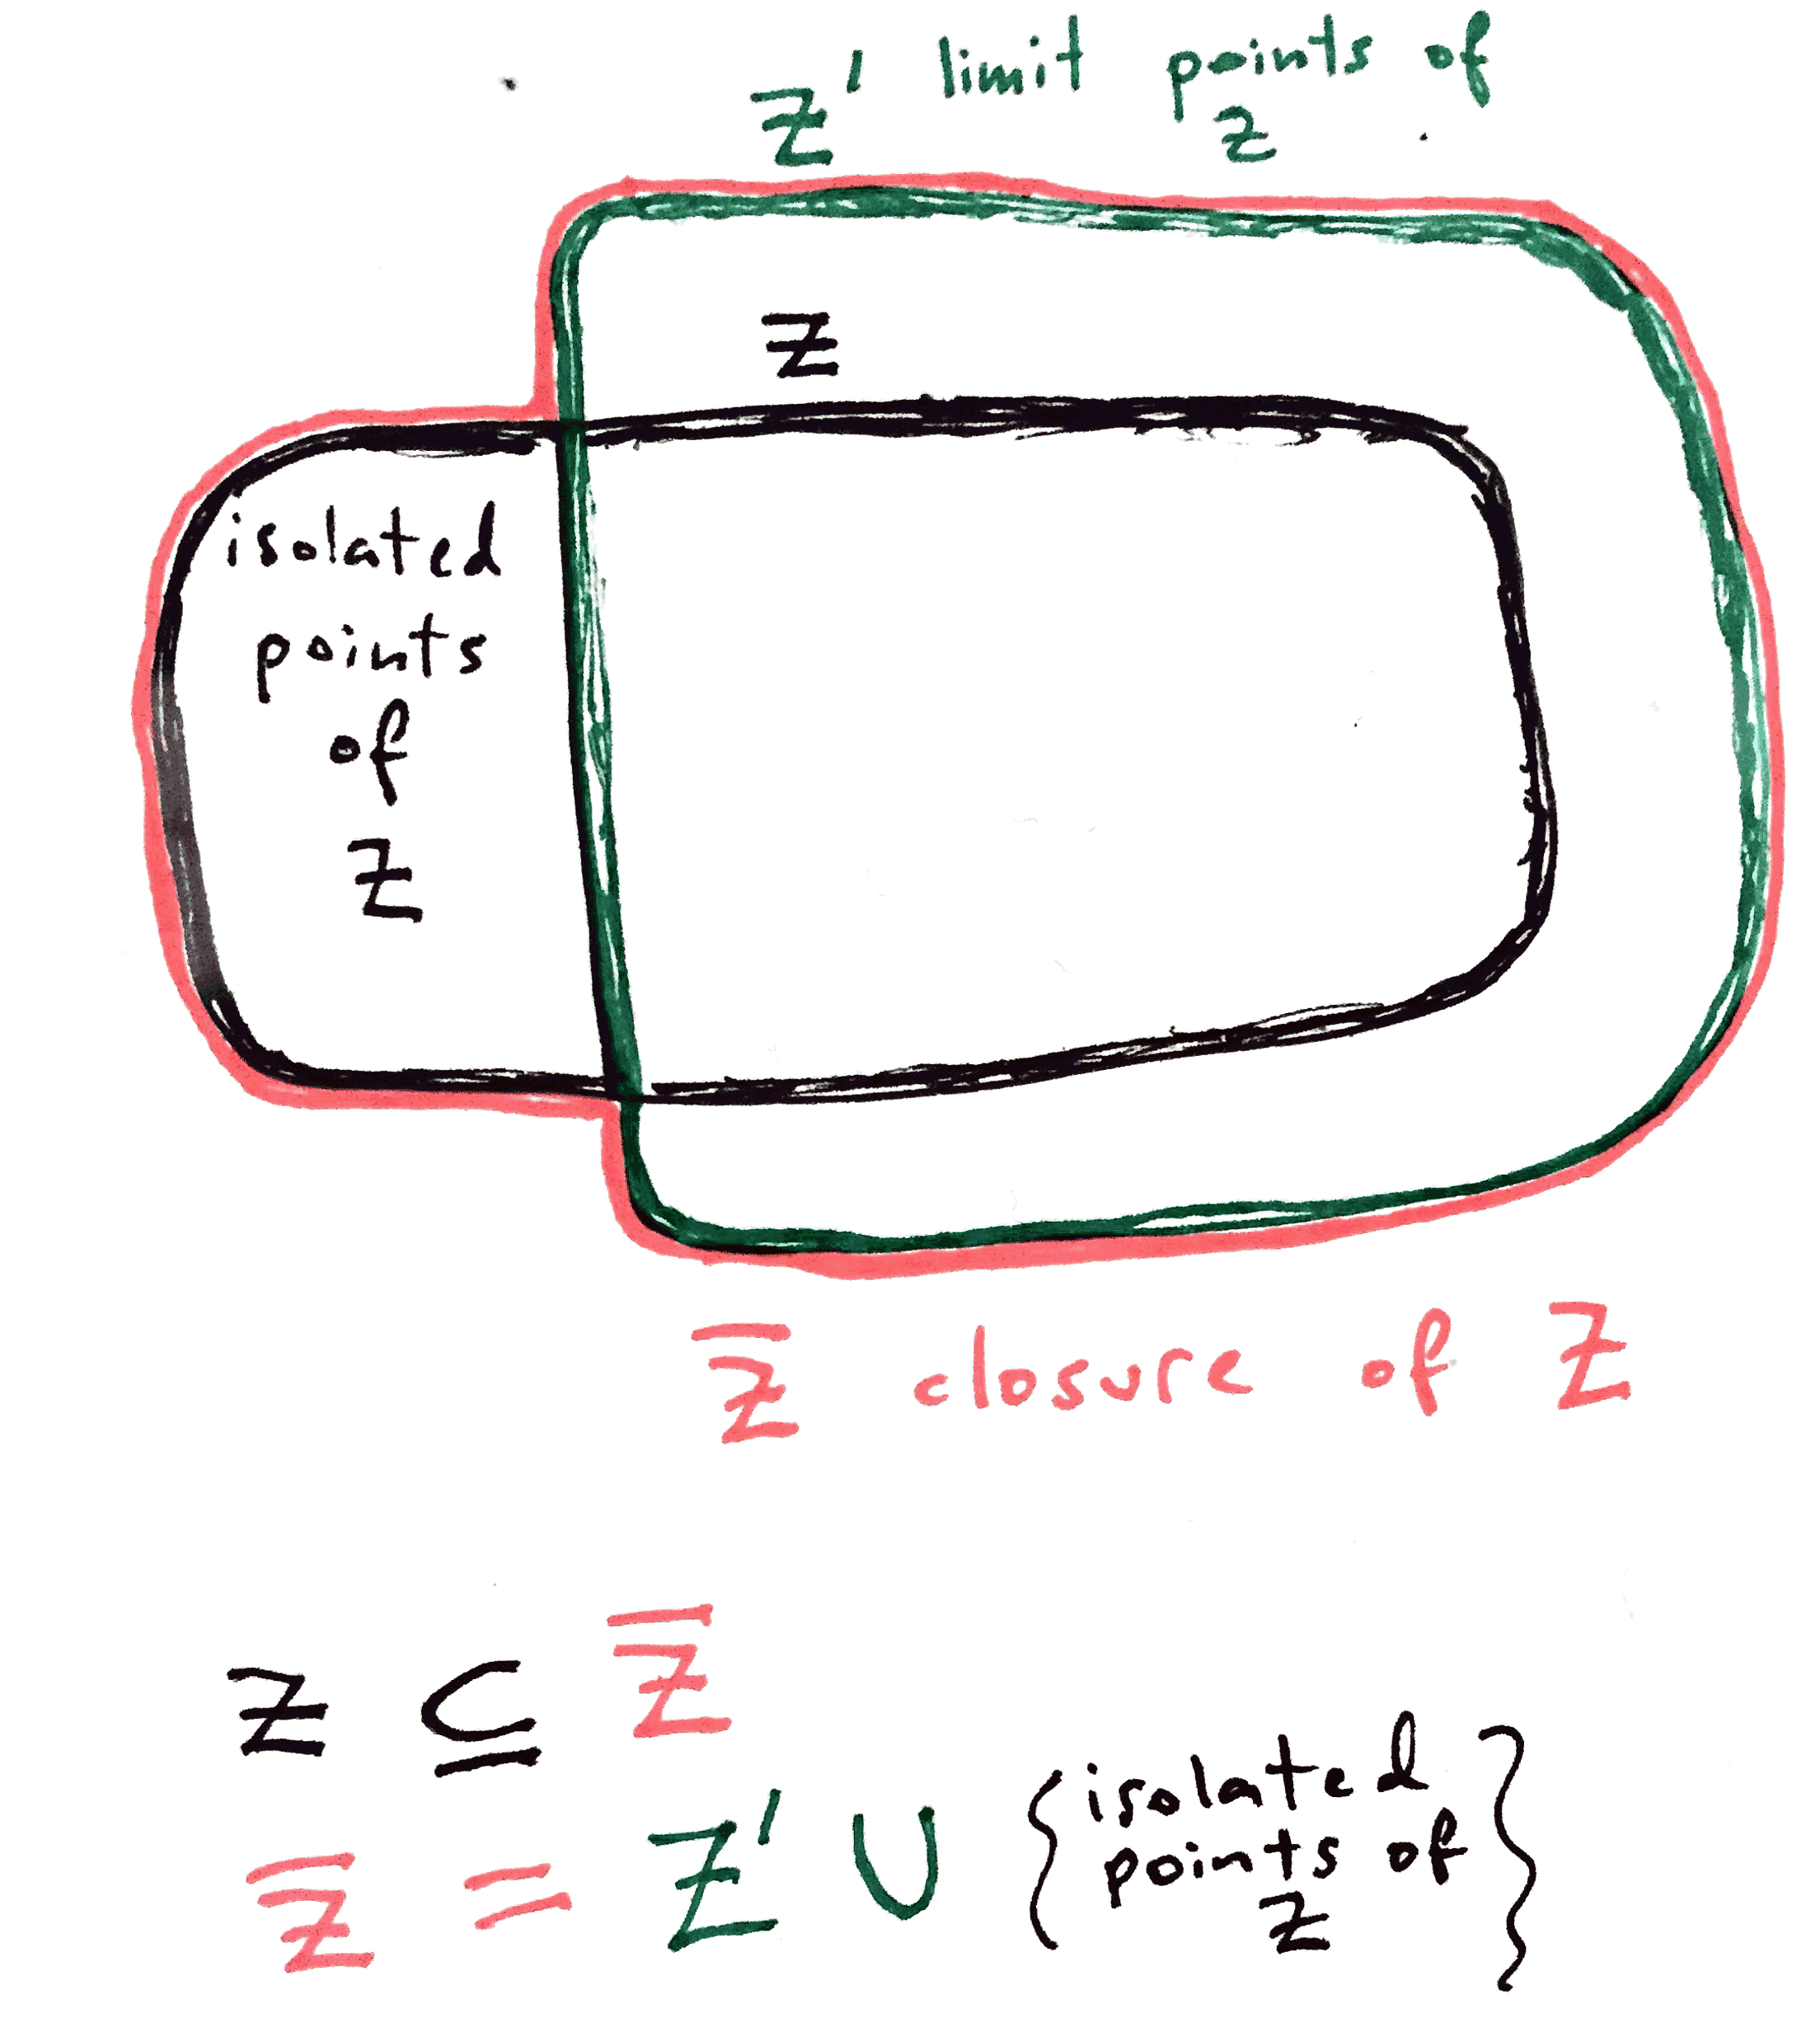
\includegraphics[width=200pt]{img/metric-space-closure-limit-points.png}
\end{mdframed}


\newpage
\subsection{Isometries and Homeomorphisms}
\begin{enumerate}
\item {\bf Definition}: An \defn{isometry} is a map between metric spaces that preserves pairwise distances. It is
  necessarily continuous and injective.
\item {\bf Definition}: A \defn{homeomorphism} is a continuous map between metric spaces that has a
  continuous inverse.
\item {\bf Definition}: Metric spaces $X$ and $Y$ are \defn{isometric} if there is a {\it
    bijective} isometry between them, and they are \defn{homeomorphic} if there is a homeomorphism
  between them.
\item {\bf Example}:
  \begin{mdframed}
    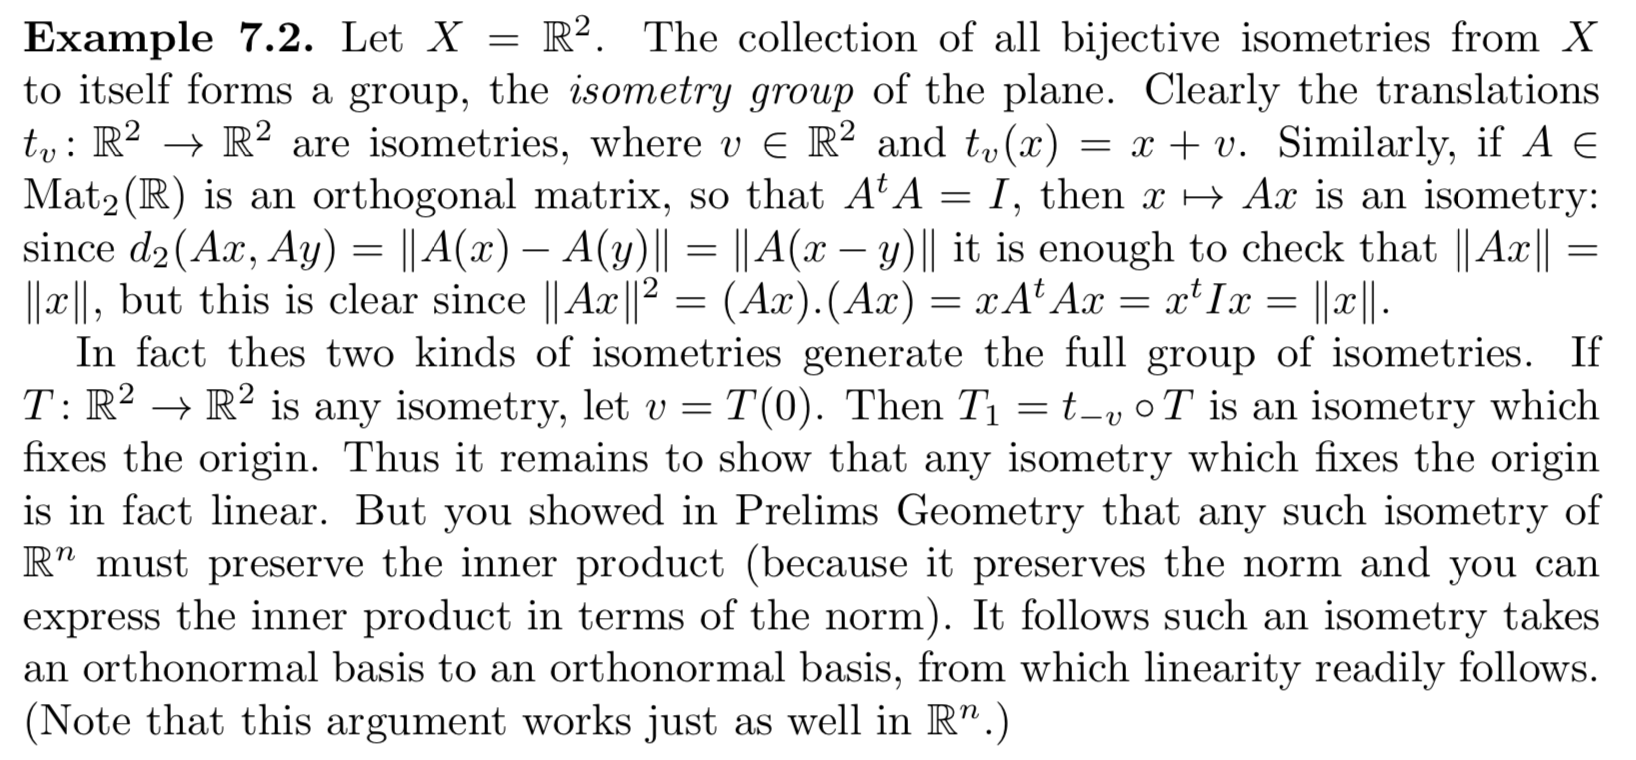
\includegraphics[width=300pt]{img/oxford-a2-isometry-group.png}
  \end{mdframed}
\end{enumerate}

\subsection{Completeness}
\begin{enumerate}
\item {\bf Definition}: A sequence is \defn{Cauchy} if for every $\epsilon > 0$ there is an $N$
  beyond which all pairs of sequence values lie within $\epsilon$ of each other.
\item {\bf Theorem}:
  \begin{enumerate}[label=(\roman*)]
  \item Convergent $\implies$ Cauchy.
  \item Cauchy $\implies$ bounded.
  \end{enumerate}
\item {\bf Definition}: A metric space $X$ is \defn{complete} if (Cauchy) $\implies$ (convergent in $X$)
\item {\bf Example}: $\R^n$ and $\C$ are complete.
\item {\bf Example}: $(0, 1]$ is not complete because $(1/n)$ is Cauchy yet converges to a point
  outside the metric space.
\item {\bf Theorem}: For a {\it subset of a complete metric space}: closed $\iff$ complete.
\item {\bf Theorem}: Consider a nested sequence of closed sets in a metric space. There is a unique
  point that is in every nested subset no matter how far the sequence is taken.
\item {\bf Theorem}: Completeness is not preserved by homeomorphism: homeomorphism does not take
  Cauchy sequences to Cauchy sequences.
\item {\bf Example}: Although $\R$ and $(0, 1)$ are homeomorphic, the former is complete while the
  latter is not. (For a homeomorphism define $f: \R \to (0, 1) $ by
  $x \mapsto \frac{e^x}{1 + e^x}$; the inverse is $p \mapsto \log(\frac{p}{1-p})$.)
\item {\bf Example}:
  \begin{mdframed}
    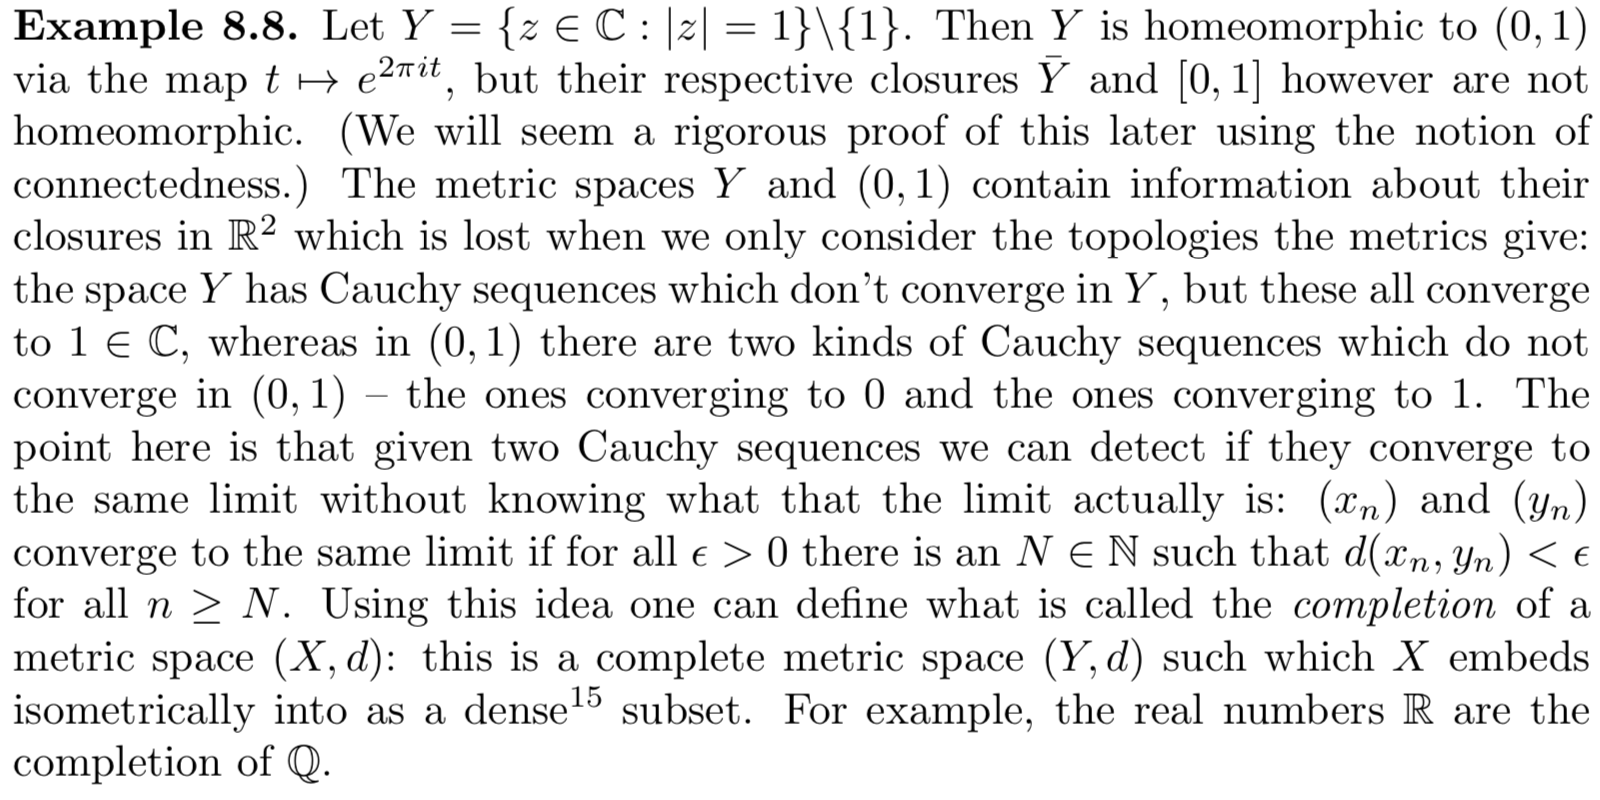
\includegraphics[width=300pt]{img/oxford-a2-completion.png}
  \end{mdframed}
\item {\bf Theorem}: Let $X$ be a set. The set $\mathcal{B}(X)$ of bounded $X \to \R$ functions
  with the $\|.\|_\infty$ norm is a complete normed vector space.
\item {\bf Theorem}: Let $(X, d)$ be a metric space. The set $\mathcal{C}_b(X)$ of bounded
  continuous functions on $X$ is a complete normed vector space.
\item {\bf Theorem} (Weierstrass M-test) The series $\sumn f_n$ of functions in $\mathcal{C}_b(X)$
  converges if there exists a sequence of real numbers $(M_n)$ such that $\|f_n\|_\infty \leq M_n$
  and $\sumn M_n$ converges. (The proof involves showing that the sequence of partial sums is
  Cauchy.)
\item {\bf Definition}: Let $X$ be a set and $Y$ be a metric space. A function $X \to Y$ is
  \defn{bounded} if there exists $K \in \R$ such that $d(f(x_1), f(x_2)) < K$ for all
  $x_1, x_2 \in X$.
\item {\bf Definition}: Let $X$ be a set. A function $X \to \R$ is \defn{bounded} if there exists
  $K \in \R$ such that $|f(x)| < K$ for all $x \in X$. \red{are these definitions consistent?} The
  set of all bounded $X \to \R$ functions is denoted $\B(X)$.
\item {\bf Definition}: A map $f:M \to N$ from one metric space to another is \defn{Lipschitz} if
  there exists $K > 0$ such that $d_N\((f(x_1), f(x_2)\) \leq K d_M(x_1, x_2)$ for all
  $x_1, x_2 \in M$.
\item {\bf Definition}: A map from a metric space to {\it itself} is a \defn{contraction} if it is
  Lipschitz with $K < 1$. \todo{Why is a contraction not defined for a map between different metric
    spaces?}
\item {\bf Theorem} (Banach Fixed Point Theorem): A contraction on a complete metric space has a
  unique fixed point. (The proof involves constructing a sequence by $x_n = f(x_{n-1})$ for some
  initial value $x_0 = a$.)
\item {\bf Theorem}:
  \begin{theorem*}
    Let $X$ be a set. The normed vector space $(\B(X), \|.\|_\infty)$ is complete.
  \end{theorem*}
  \begin{remark*}
    The key in this proof is that the $d_\infty$ metric implies
    $|f_m(x) - f_n(x)| \leq \|f_m - f_n\|$ for all $x \in X$. This allows a single $\epsilon$
    obtained in $\B(X)$ under $d_\infty$ to apply for all values of $x \in X$ under the $|.|$
    metric in $\R$, in a manner reminiscent of uniform convergence.
  \end{remark*}
  \begin{proof}~\\
    Let $(f_n)$ be a Cauchy sequence in $\B(X)$. We want to show that $(f_n)$ converges in $\B(X)$.

    For all $x \in X$ we have
    $|f_m(x) - f_n(x)| \leq \|f_m - f_n\|_\infty \to 0 ~\text{as}~ m, n \to \infty$.

    Therefore $(f_n(x))$ is Cauchy in $\R$, and therefore converges in $\R$.

    Define $f(x) = \limn f_n(x)$ for all $x \in X$. We claim that $f_n \to f$ and that
    $f \in \B(X)$.

    Fix $\epsilon > 0$. Let $N$ be such that
    $|f_m(x) - f_n(x)| \leq \|f_m - f_n\|_\infty < \epsilon$ for all $x \in X$ and for all
    $m, n > N$.

    Letting $m \to \infty$ we have $|f(x) - f_n(x)| \leq \|f - f_n\|_\infty < \epsilon$ for all
    $x \in X$ and for all $n > N$. Therefore $f_n \to f$ as claimed, and also $f - f_n \in
    \B(X)$. But $\B(X)$ is a vector space, so $f = f_n + (f - f_n) \in \B(X)$.
  \end{proof}


\end{enumerate}

\newpage
\subsection{Connectedness}
\begin{enumerate}
\item {\bf Definition}: A set is \defn{disconnected} if it can be written as the union of {\it two
    nonempty open subsets with empty intersection}. Note that, since they are the complement of
  each other, the two subsets are also closed.  A set is \defn{connected} if it is not
  disconnected.
\item {\bf Example}:
  \begin{enumerate}[label=(\roman*)]
  \item $[0, 1) \cup (1, 2]$ is disconnected (despite the square brackets, both subsets are open in
    $[0, 2]$.)
  \item $[0, 1] \cup (1, 2]$ is connected.
  \end{enumerate}
\item {\bf Theorem}: $\R$ is connected.\\
  {\it Intuition}: Basically you can't partition $\R$ into two non-empty disjoint open sets because
  the supremum of one of the sets would be left out.
  \begin{proof}
    Let $U, V$ be disjoint open sets such that $U \cup V = \R$. Suppose for a contradiction that
    neither is empty. Let $x \in U$ and $y \in V$ where WLOG $x < y$. Let
    $S = \{z ~|~ [x, z] \subseteq U\}$, and let $c = \sup S$. Then $c \notin U$ (since the
    Approximation Property of the supremum would allow us to exhibit $c < d \in U$, contradicting
    $c$ as supremum of $S$). Also $c \in V$ leads to a contradiction since we would be able to
    exhibit $c > d \in V$ so that $d$ would be a lower upper bound of $S$ than $c$. Hence either
    $U$ or $V$ is empty.
  \end{proof}
\item {\bf Definition}: a metric space is \defn{discrete} if every point is the sole member of a
  singleton open set.
\item {\bf Theorem}:
  \begin{enumerate}[label=(\roman*)]
  \item
    ($X$ connected) $\iff$\\
    ($f:X \to$ (discrete space) continuous $\implies$ $f$ constant) $\iff$\\
    ($X$ and $\emptyset$ are the only open and closed subsets)
  \item If a collection of connected subsets have non-empty intersection, then their union is
    connected.
  \item If $A$ is connected and $B \subseteq \bar A$, then $B$ is connected.
  \item The image of a connected set under a continuous map is connected. (Therefore if two metric
    spaces are homeomorphic then they are either both connected or both disconnected.)
  \end{enumerate}
\item {\bf Definition}: The \defn{connected component} containing $x_0$ is the union of all connected sets
\item {\bf Theorem} (Intermediate Value Theorem): If $f: [a, b] \to \R$ is continuous, then its
  image is the connected set $[f(a), f(b)]$, and therefore $f$ hits every value in that interval.
\item {\bf Definition}: A \defn{path} is a continuous function $[0, 1] \to X$. A subset is
  \defn{path connected} if there is a path between every pair of points.
\item {\bf Theorem}:
  \begin{enumerate}[label=(\roman*)]
  \item (path connected) $\implies$ (connected)
  \item (path connected) $\impliedby$ (connected) for an open subset of a normed vector space.
  \end{enumerate}
\item {\bf Example} of a subset that is {\it connected but not path connected}: let
  $A = \{(t, \sin(1/t))~|~t \in (0, 1)\}$. The closure is $\bar A = A \cup \{0\} \times [-1,
  1]$.\\
  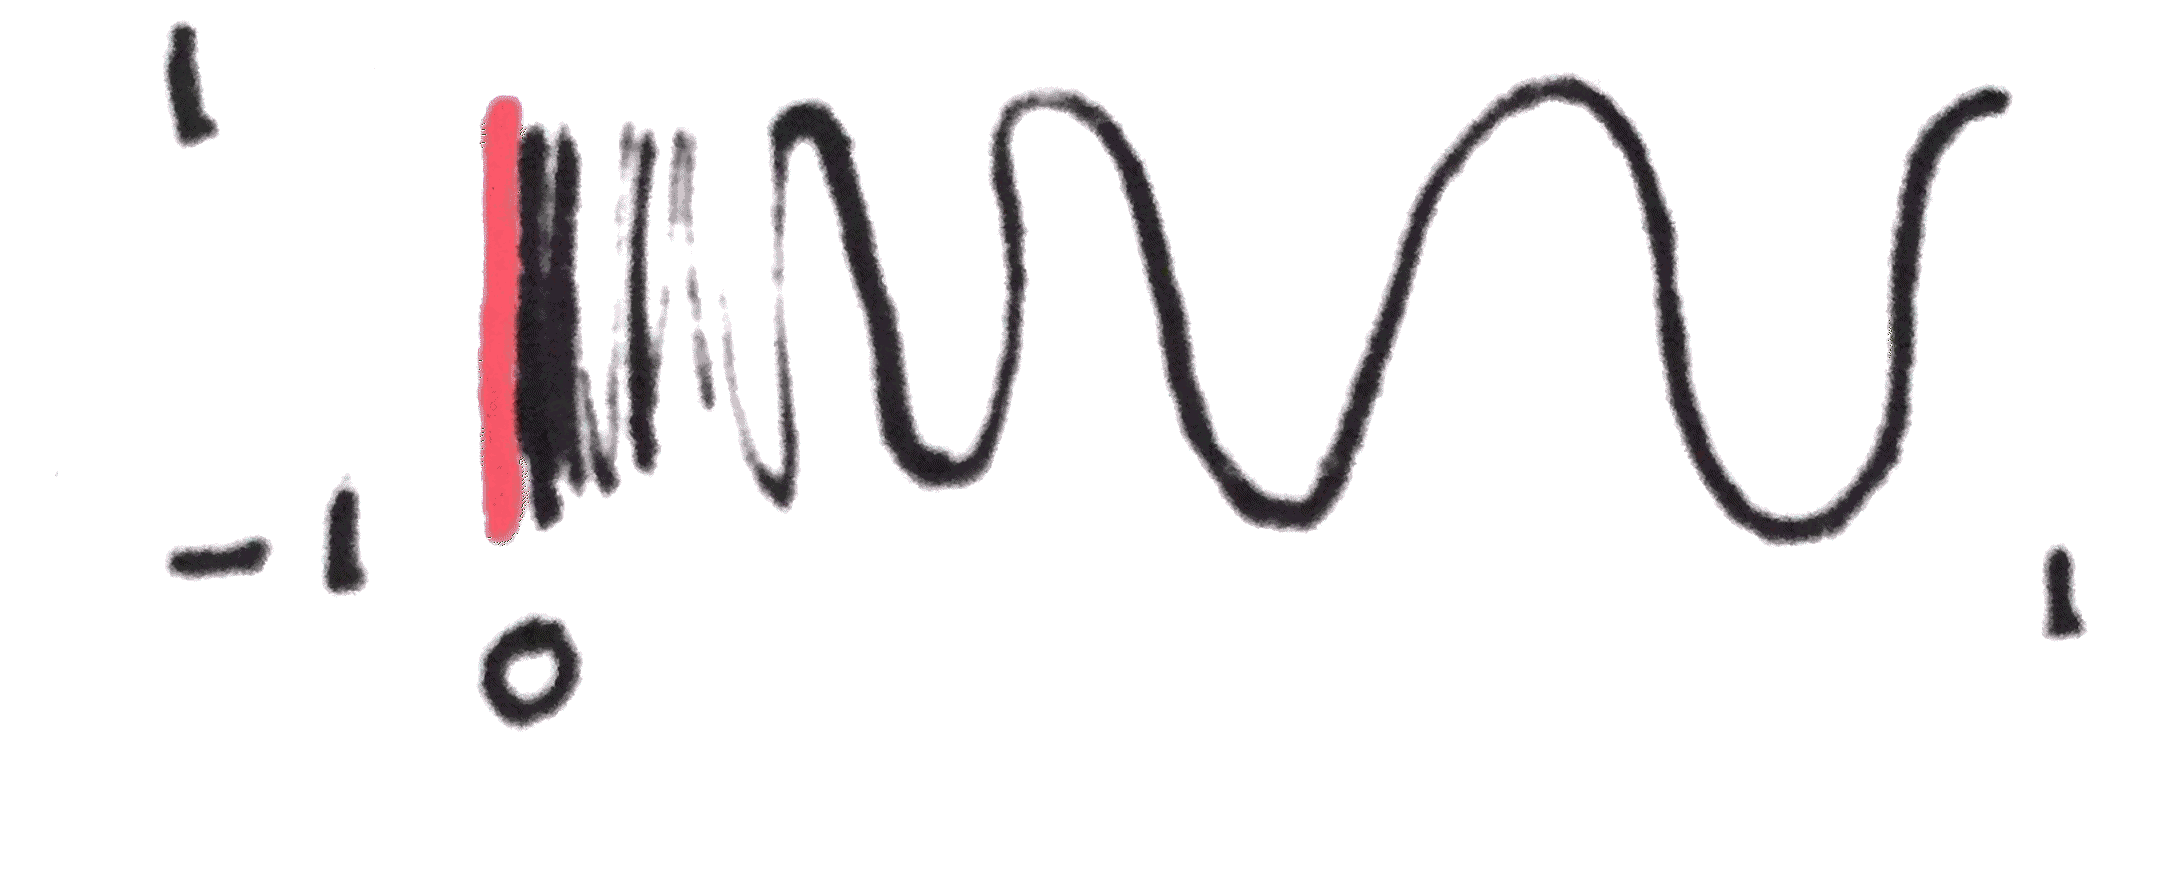
\includegraphics[width=100pt]{img/oxford-a2-connected-not-path-connected.png}\\
  This is connected (since it's the image of a connected set under a continuous map), but
  (claim) it is not path connected.

\subsection{Compactness}
\item {\bf Definition}: An \defn{open cover} of a set is a collection of open sets whose union
  equals the set. A \defn{subcover} is a subset of a cover that still covers. Covers and subcovers
  may be finite or non-finite.
\item Suppose $\{U_1, U_2, \ldots\}$ is an open cover. A property $P$ of a function $f$ is \defn{local} if\\
  ($P$ is true for all $f_{|U_i}$) $\iff$ ($P$ is true everywhere)\\~\\
  {\bf Local properties}: continuity, differentiability\\
  {\bf Global properties}: boundedness (e.g. $x \mapsto 1/x$: local restrictions are bounded while
  the function is not.)
\item {\bf Definition}: A set is \defn{compact} if every open cover has a finite subcover.
\item Equivalently, $A \subseteq X$ is compact if, whenever $A$ is a subset of a union of open sets
  in $X$, it is also a subset of some {\it finite} union of those open sets.
\item {\bf Theorem}
  \begin{enumerate}[label=(\roman*)]
  \item $(0, 1)$ is not compact: an open cover is $\bigcup_{n \geq 2} (1/n, 1)$ but this has no
    finite subcover.
  \item Heine-Borel: $[a, b]$ is compact. (A proof is by contradiction: suppose there is an open
    cover with no finite subcover. It involves constructing a sequence of nested closed
    subintervals that would similarly have an open cover with no finite subcover. But since we are
    working in a complete metric space, there is a unique point that remains in such an
    indefinitely long sequence of nested closed subsets; this results in an interval that
    necessarily would have a finite subcover - contradiction.)
  \end{enumerate}
\item {\bf Theorem}: Under a continuous map:
  \begin{enumerate}[label=(\roman*)]
  \item The preimage of an open / closed set is open / closed respectively.
  \item The image of a connected / compact set is connected / compact respectively.
  \item Therefore connectedness and compactness are preserved by homeomorphism.
  \end{enumerate}
\item {\bf Theorem}
  \begin{enumerate}[label=(\roman*)]
  \item (compact) $\implies$ (closed and bounded)
  \item For a subset of a compact set (closed) $\iff$ (compact)
  \item The image of a compact set under a continuous function is bounded, and the function attains
    its bounds (equivalent to saying the image is closed and bounded?).
  \end{enumerate}
\item {\bf Theorem} A continuous bijection from a compact metric space to another metric space is
  automatically a homeomorphism.
  \begin{proof}
    Let $f: X \to Y$ be a continuous bijection between compact metric spaces. We will show that
    $f^\1$ is continuous by showing that the preimage under $f^\1$ of a closed set is closed.
    Consider closed $Z \subseteq X$. Note that $f(Z)$ is the preimage of $Z$ under $f^\1$ . $Z$ is
    compact since it is a closed subspace of a compact space. Therefore $f(Z)$ is compact since $f$
    is continuous. Therefore $f(Z)$ is closed since it is a compact subspace of a compact space.
  \end{proof}
\item {\bf Theorem}: The product of two compact spaces is compact.
\item {\bf Theorem} (Heine-Borel): $X \subset \R^n$ is compact iff it is closed and bounded.
  \begin{proof}
    We've already shown that (compact) $\implies$ (closed and bounded); we need to show (closed and
    bounded) $\implies$ (compact). Let $X \subset \R^n$ be closed and bounded. We've already shown
    that $[a, b]$ is compact. Note that there exists $r > 0$ such that $X \subseteq [-r, r]^n$. But
    then since the product of compact spaces is compact, we have $X$ a closed and bounded subset of
    a compact space and therefore compact.
  \end{proof}
\item {\bf Theorem} Every continuous function on a compact metric space is uniformly continuous.
\item {\bf Definition}: A \defn{sequentially compact} space is a metric space in which every
  sequence has a convergent subsequence.
\item {\bf Theorem} (compact) $\iff$ (sequentially compact). Note
  \begin{enumerate}[label=(\roman*)]
  \item Bolzano-Weierstrass shows that a closed interval in $\R$ is sequentially compact.
  \item This course proves the forward implication only.
  \end{enumerate}
\item (compact) $\implies$ (complete)
\item {\bf Definition}: a metric space is \defn{totally bounded} if it can be formed as a union of
  a finite number of open balls of radius $\epsilon$, for all $\epsilon > 0$.
\item {\bf Theorem}: (compact) $\iff$ (sequentially compact) $\iff$ (closed and totally bounded)
\item {\bf Theorem}: consider a compact subset of an open subset of a metric space. There exists an
  $\epsilon > 0$ such that at every point of the compact subset an open ball can be placed that
  remains within the enclosing open subset.
\item~\\
  \begin{mdframed}
    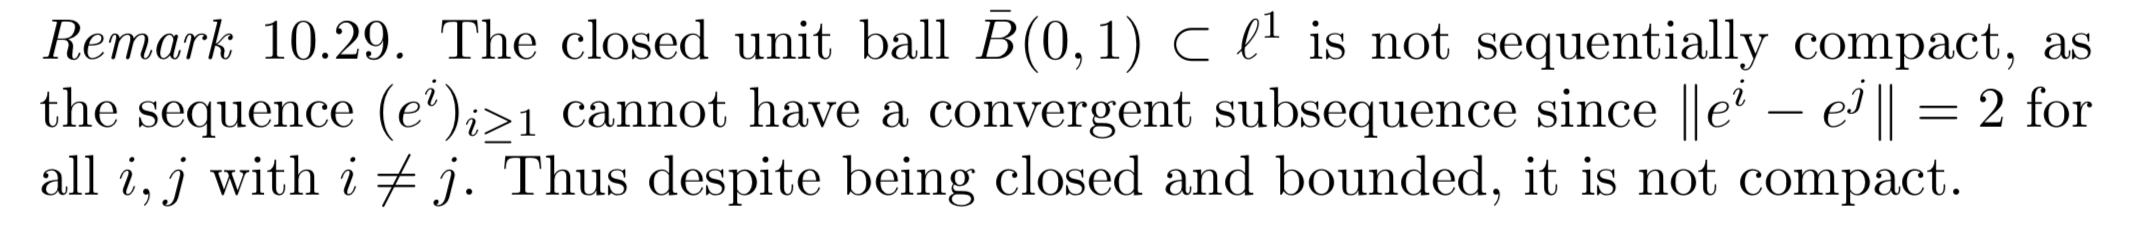
\includegraphics[width=400pt]{img/oxford-a2-compactness-counterexample.png}
  \end{mdframed}
  \begin{mdframed}
    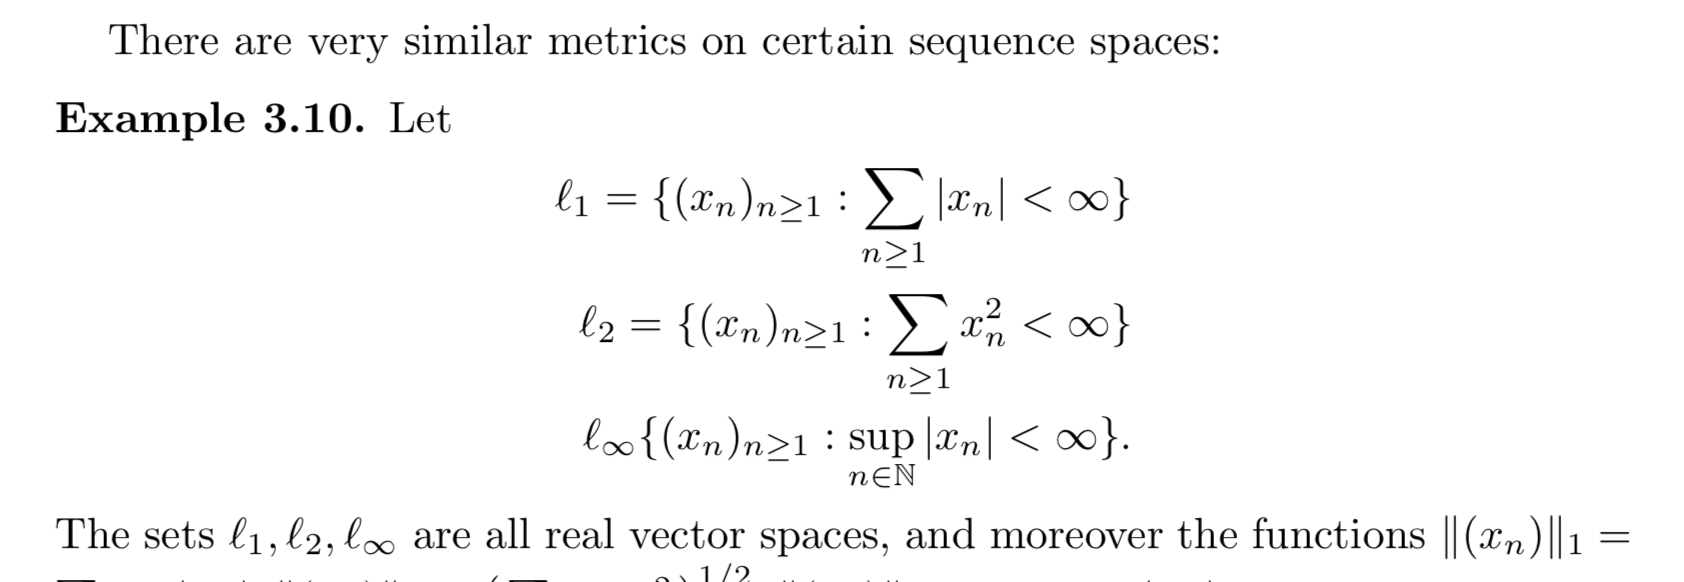
\includegraphics[width=400pt]{img/oxford-a2-compactness-counterexample-2.png}
  \end{mdframed}
\end{enumerate}

\newpage


The following subsections are older notes on metric spaces.
\subsection{Metric space}
\begin{definition}
  Let $X$ be a set. Suppose $d:X \times X \to \R$ satisfies positivity, symmetry and the triangle
  equality. Then $d$ is a metric and $(X, d)$ is a metric space.
\end{definition}

\subsection{Open ball}
\begin{definition}
  Let $(X, d)$ be a metric space, $x \in X$ and $\delta > 0$. Then
  $B(x, \delta) := \{x \in X ~|~ d(x, x) < \delta\}$ is an open ball of radius $\delta$ centred at
  $x$.
\end{definition}

\begin{remark*}
  Note that a ball in $X$ might ``push up against'' the boundary of $X$, in which case it will be
  ``flattened'' on that side, and thus not ``spherical''.

  Also closed ball, $\leq$. E.g. singleton set.
\end{remark*}

\subsection{Ball-based continuity criterion}
\begin{lemma}
  $f$ is continuous at $x$ if for all $\epsilon > 0$ there exists $\delta > 0$ such that
  $f\(B(x, \delta)\) \subseteq B(f(x), \epsilon))$.

  Equivalently, $B(x, \delta) \subseteq f^\1\(B(f(x), \epsilon)\)$.
\end{lemma}

\subsection{Neighbourhood}
\begin{definition}
  Let $(X, d)$ be a metric space. $N \subseteq X$ is a neighbourhood of $x \in X$ if there exists
  $\delta > 0$ such that $B(x, \delta) \subseteq N$.
\end{definition}

\begin{remark*}
  $N$ is a neighbourhood of $x$ if a ball can be placed at $x$ without poking outside $N$.
\end{remark*}

\begin{theorem*}[Neighbourhoods are open]
  Let $(X, d)$ be a metric space and let $N \subseteq X$ be a neighbourhood of $x \in X$. Then $N$
  is open.

  \red{I don't think they are under the definitions here.}
\end{theorem*}

\begin{proof}
  Let $N = \{x' \in X ~|~ d(x, x') \leq 1\}$. Then $N$ is a neighbourhood of $x$ since
  $B(x, 0.5) \subset N$. But $N$ is not open.
\end{proof}


% \begin{proof}
%   Let $N \subseteq X$ be a neighbourhood of $x \in X$ and let $n \in N$. We wish to show that there
%   exists $\delta$ such that $B(n, \delta) \subseteq N$.

%   Since $N$ is a neighbourhood of $x$ there exists $\epsilon$ such that
%   $B(x, \epsilon) \subseteq N$.

%   Suppose $n \in B$.
% \end{proof}

\subsection{Open and closed subsets of a metric space}
\begin{definition}
  Let $(X, d)$ be a metric space. Then $U \subseteq X$ is open if it is a neighbourhood of all of
  its elements.

  $V \seq X$ is closed iff its complement in $X$ is open.
\end{definition}


\subsection{Examples}


Let $X = [0, 1) \cup \{2\}$ and
\begin{align*}
f(x) =
\begin{cases}
  x, ~~~~~~~ 0 \le x < 1 \\
  1, ~~~~~~~ x = 2
\end{cases}
\end{align*}


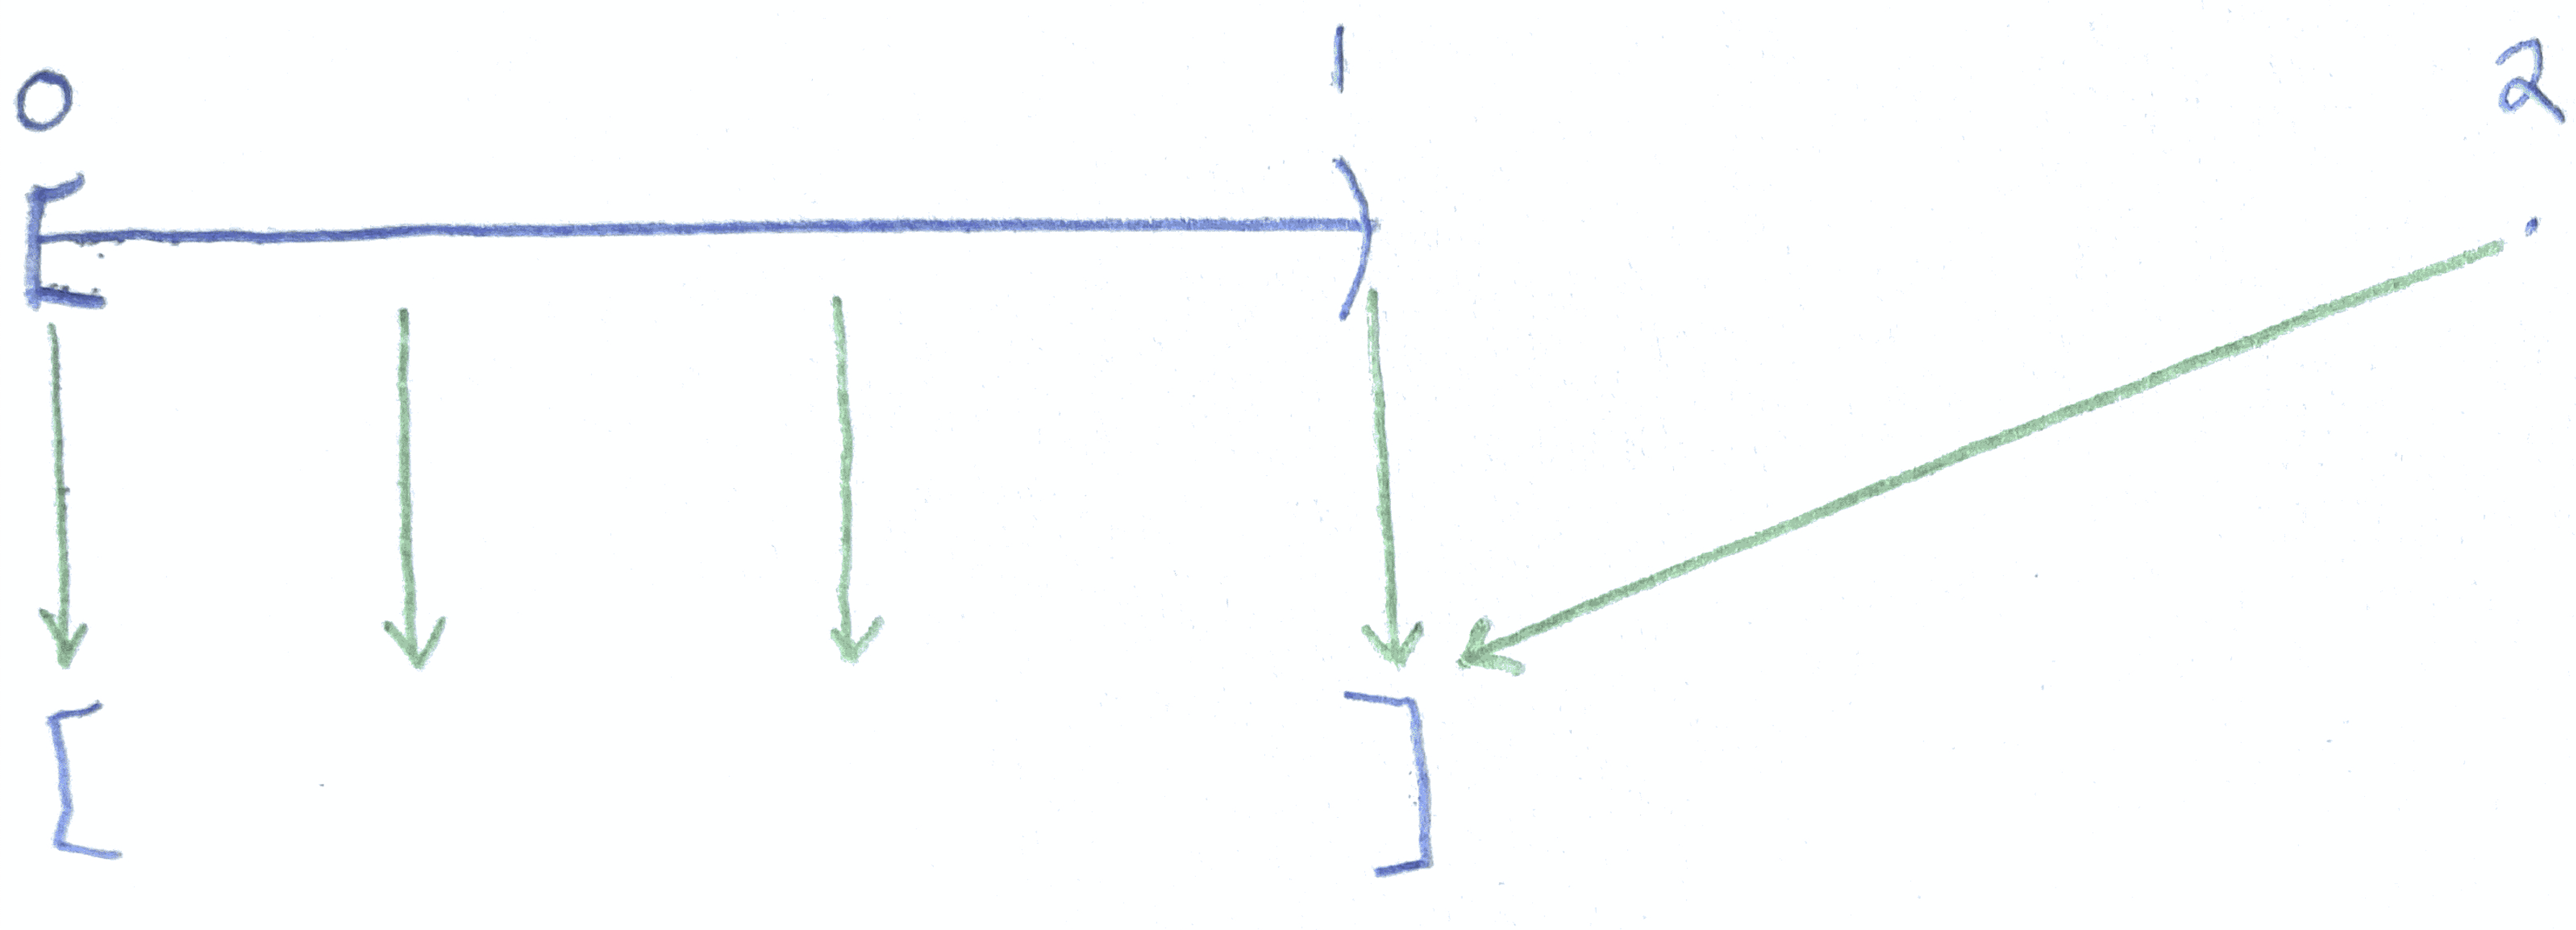
\includegraphics[width=400pt]{img/analysis--real-analysis--examples-083a.png}

\begin{itemize}

\item The limit of $f(x)$ as $x \to 1$ is 1.
  \begin{itemize}
  \item Recall $f(x) \to L$ if $L$ is the limit of $f(x_1), f(x_2), \ldots$ for {\it every} sequence that converges to 1.
  \item Since $1 \notin X$, the sequences that converge to 1 never hit 1, but satisfy the standard $\epsilon-N$
    criterion: for any $\epsilon$ there exists an $N$ such that the sequence remains within $\epsilon$ of 1
    beyond $N$.
  \item The limit of the function values is 1 since, for any $\epsilon$, beyond a certain point, we remain
    within $\epsilon$ of 1. That point is whenever the sequence in the domain gets within $\epsilon$ of 1.
  \end{itemize}

\item 1 is not in the domain of $f$, so we cannot ask whether $f$ is continuous at 1.

\item The only sequences that converge to 2 are those with a constant tail of infinitely many 2s.

\item The limit of $f(x)$ as $x \to 2$ is also 1.

\item Ball-based definition of continuity: $f$ is continuous at $a$ if for any $\epsilon$ there exists a
  $\delta$ such that an open ball of radius $\delta$ centred at $a$ has as image a subset of the open ball of
  radius $\epsilon$ centred at $f(a)$.

\item Topological definition of continuity: $f$ is continuous at $a$ if the preimage of every open set
  containing $f(a)$ is an open set in $X$?


\end{itemize}

Note:


\begin{enumerate}
\item $f(x) \to L$ as $x \to a$ if for all $\epsilon$ there exists $\delta$ such that $d(x, a) < \delta \implies d(f(x), L) < \epsilon$.
\item Equivalently, if the limit of the sequence of function values is $L$ for every sequence in the domain that
  converges to $a$.
\item $f(x)$ is continuous at $a$ if $L = f(a)$.
\end{enumerate}


d(X,Y) = size of the set containing elements in X xor Y
“measure of the symmetric difference b/w X and Y"




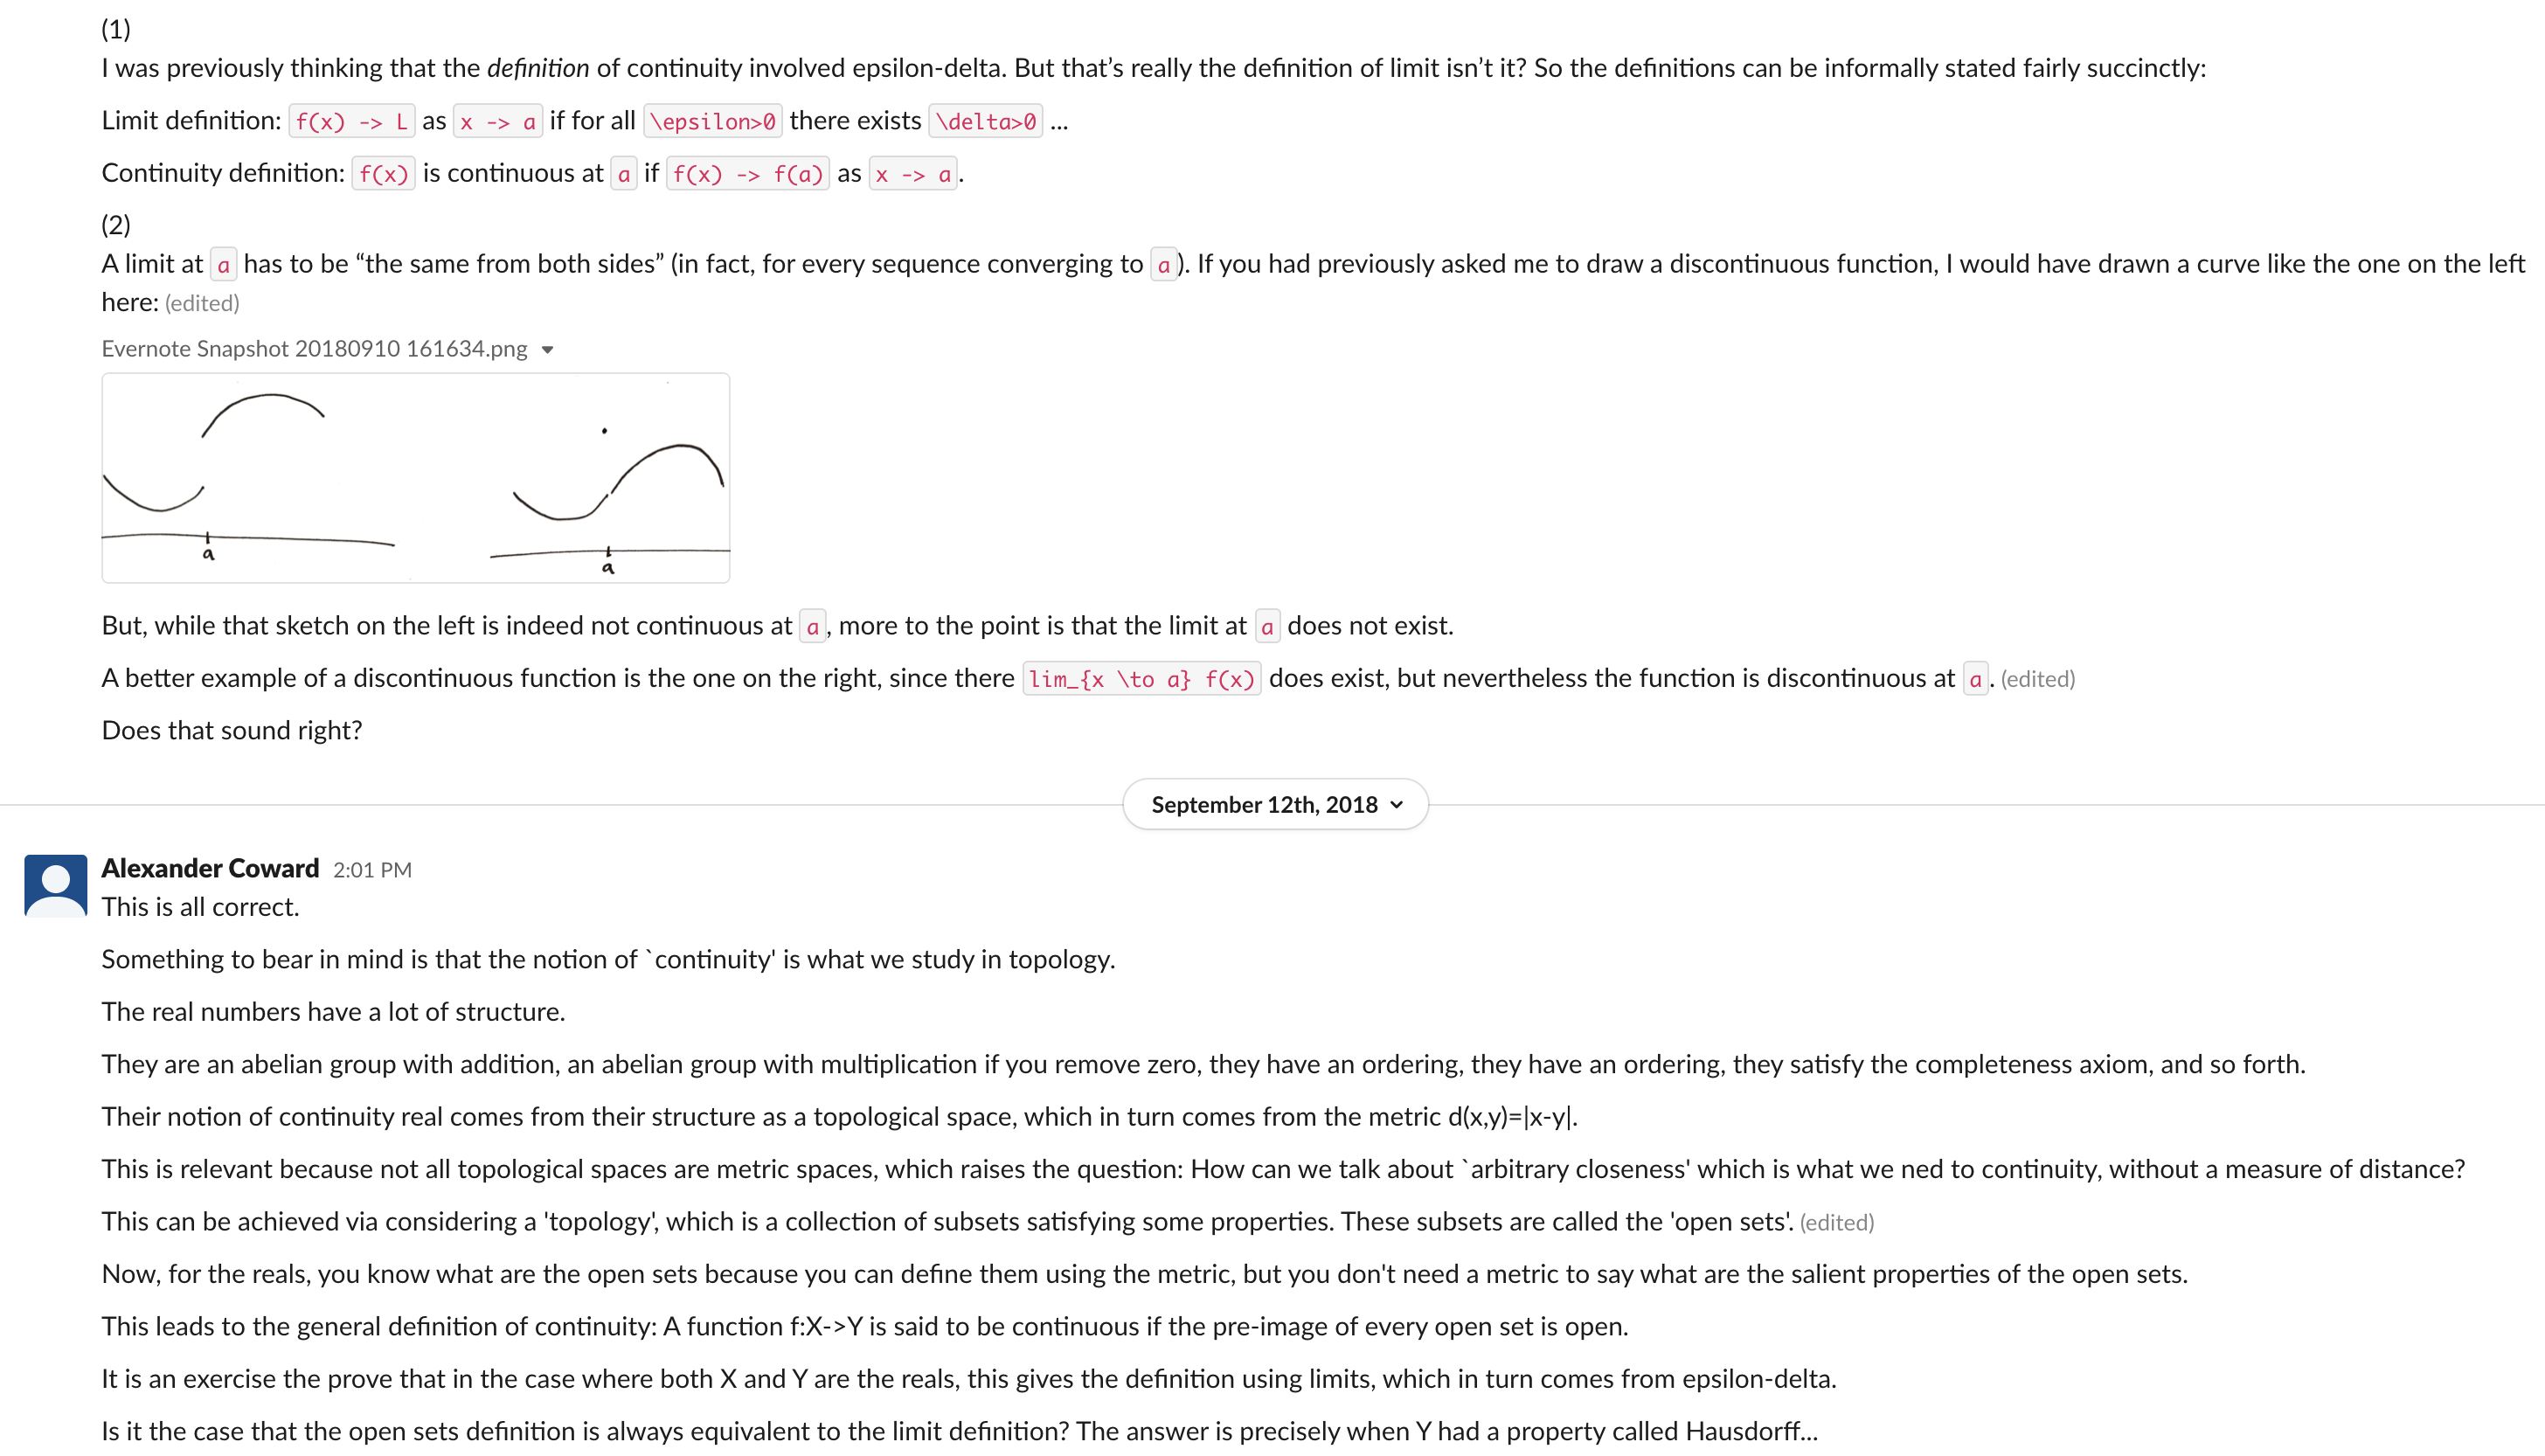
\includegraphics[width=400pt]{img/analysis--real-analysis--examples-58e8.png}

h
\subsection{Topology on a metric space}
\begin{definition}
  Let $(X, d)$ be a metric space. The collection $\mc T$ of all open sets in the metric space is
  called the topology of $X$.
\end{definition}

\begin{remark*}
  Note that the definitions so far have the following dependency:

  (open set) $\larrow$ (neighbourhood) $\larrow$ (ball) $\larrow$ (metric),

  so they apply to metric spaces only.
\end{remark*}

\subsection{Open set-based continuity criterion}
\begin{theorem}
  Let $X$ and $Y$ be metric spaces and let $f:X \to Y$. Then

  $f$ is continuous at $x$ iff for every neighbourhood $N \subseteq Y$ of $f(x)$, the preimage
  $f^\1(N)$ is a neighbourhood of $x \in X$.

  $f$ is continuous iff for every open set $U$ of $Y$, $f^\1(U)$ is an open set of $X$.
\end{theorem}

\begin{remark*}
  So we have defined continuity in terms of open sets (the topology). This means that the metric is
  only relevant insofar as it induces the topology; two metric spaces with the same topology have
  the same notion of continuity.
\end{remark*}

\begin{proof}~\\
  Let $f$ be continuous at $x \in X$, and let $N \seq Y$ be a neighbourhood of $f(x)$.

  Then by definition of neighbourhood there exists a ball at $f(x)$ that stays within $N$.

  By continuity of $f$ the preimage of that ball is a superset of a ball at $x$.

  So the preimage of the ball is a neighbourhood of $x$. Therefore the preimage of $N$ is also.

  Conversely, ... similar.

  Let $f$ be continuous on $X$. Now every open set $U$ of $Y$ contains a ball around some point $y$...
\end{proof}

\subsection{Topology on a set, topological space}
\begin{definition}
  A topology on a set $X$ is a collection $\mc T$ of subsets of $X$, which are called the \defn{open sets}. They must
  satisfy
  \begin{enumerate}
  \item closed under arbitrary unions. In particular, $\emptyset$ is an open set of $X$.
  \item closed under finite intersections. In particular, $X$ is an open set of $X$.
  \end{enumerate}
  A topological space is a pair $(X, \mc T)$.
\end{definition}

\begin{remark*}
  Criteria for closed sets follow by applying de Morgan's laws (closure under finite unions and
  arbitrary intersections).

  $f:X\to Y$ closed iff $f^\1(V)$ is closed for all closed sets $V \seq Y$.
\end{remark*}

\subsection{Limit point}
\begin{definition}
  Let $(X, d)$ be a metric space and $Z \seq X$ be any subset.

  $x \in X$ is a limit point of $Z$ if for all $\delta > 0$ the deleted open ball
  $B(x, \delta)\setminus\{x\}$ has non-empty intersection with $Z$.

  If $z \in Z$ is not a limit point of $Z$, then it is an isolated point.

  The set of limit points of $Z$ is denoted $Z'$, and it is clear that
  $Z_1 \seq Z_2 \implies Z_1' \seq Z_2'$.
\end{definition}

\begin{intuition*}
  $x \notin Z$ is a limit point of $Z$ iff it ``touches'' $Z$.

  $z \in Z$ is a limit point of $Z$ if it ``lies in a contiguous region of $Z$''

  An isolated point of $Z$ is what it sounds like.
\end{intuition*}

\begin{example*}~\\
  Let $Z = (0, 1] \cup \{2\}$.

  Intuitively, 0 is a limit point of $Z$ because it ``touches'' $Z$.

  Formally, 0 is a limit point of $Z$ because for all $\delta > 0$ the deleted open ball
  $B(0, \delta)$ contains a point $z > 0 \in Z$.

  Intuitively, 2 is an isolated point.

  Formally, 2 is not a limit point because $\(B(2, 0.5)\setminus\{2\}\) \cap Z = \emptyset$. And
  yet $2 \in Z$, therefore 2 is an isolated point.
\end{example*}

\subsection{Open sets theorems}
\begin{enumerate}
\item An open ball is open
\end{enumerate}

\subsection{Closed sets theorems}
\begin{enumerate}
\item A closed ball is closed
\end{enumerate}


\subsection{Continuity theorems}
\begin{enumerate}
\item $f:X \to Y$ is continuous if for every open ball in $Y$ there is an open ball in $X$ that
  maps inside it.
\item $f:X \to Y$ is continuous if the preimage of $B(f(x), \epsilon)$ in $Y$ is a ball
  $B(x, \delta)$ in $X$.
\item $f:X \to Y$ is continuous if the preimage of the neighbourhood of $f(x)$ is a neighbourhood
  of $x$.
\item $f:X \to Y$ is continuous if the preimage of every open set in $Y$ is an open set in $X$.
\end{enumerate}


\subsection{Continuity of a linear map}
\begin{theorem}
  Let $f:V \to W$ be a linear map between normed vector spaces. Then $f$ is continuous if and only
  if $\{\norm{f(x)} : \norm{x} \leq 1\}$ is bounded.
\end{theorem}

\begin{proof}~\\
  Let $v \in V$.

  Note that $f(v) = f(v) - f(0)$ since $f$ is linear.

  Suppose $f$ is continuous. Then it is continuous at 0.

  Therefore for every $\epsilon > 0$ there exists $\delta > 0$ such that
  $\norm{v} < \delta \implies \norm{f(v)} < \epsilon.$

  $\vdots$

  For the converse, suppose that $\norm{v} \leq 1 \implies \norm{f(v)} < M$.

  Let $\epsilon > 0$ be given.

  Pick $\delta > 0$ such that $\delta M < \epsilon$.

  Now consider two points $u, v \in V$ where $\norm{u - v} < \delta$. We have
  \begin{align*}
    \norm{f(u) - f(v)} = \norm{f(u - v)} = \delta\norm{f\(\frac{u - v}{\delta}\)}.
  \end{align*}

  Note that $\norm{\frac{u - v}{\delta}} < 1$, therefore $\norm{f\(\frac{u - v}{\delta}\)} <
  M$. Therefore we have
  \begin{align*}
    \norm{f(u) - f(v)} < \delta M < \epsilon
  \end{align*}
  as required.
\end{proof}

\subsection{Norm of linear map is bounded}
\begin{theorem}
  $\{\norm{f(x)} : \norm{x} \leq 1\}$ is bounded for linear map $f$, under the Euclidean norm
  $\norm{}_2$.
\end{theorem}

\begin{proof}
  See Oxford A2 Sheet 1 exercises.
\end{proof}

\section{Topology}
[Oxford Part A 5]



\begin{theorem*}
  Let $f:\R \to \R$. The following are equivalent:
  \begin{enumerate}
  \item $f$ is continuous.

  \item For all open $U \subseteq \R$ we have that $f^\1(U)$ is open.
  \end{enumerate}
\end{theorem*}

\begin{proof}~\\

  By the definition of continuity we can rewrite (1) as
  \begin{enumerate}
  % \item For all $x \in \R$, for all $\epsilon > 0$, there exists $\delta > 0$ such that
  %   $|x' - x| < \delta \implies |f(x') - f(x)| < \epsilon$.
  \item For all $x \in \R$, for all $\epsilon > 0$, there exists $\delta > 0$ such that
    $f(B(x, \delta)) \subseteq B(f(x), \epsilon)$.
  \end{enumerate}\hspace{0pt}

  $(1) \implies (2)$:

  Suppose $f$ is continuous, and let $U \subseteq \R$ be open.

  If $f^\1(U) = \emptyset$ then $f^\1(U)$ is open.

  Alternatively, let $x \in f^\1(U)$. We must show that there exists $\delta > 0$ such that
  $B(x, \delta) \subseteq f^\1(U)$.

  We know that $f(x) \in U$. Furthermore, since $U$ is open, there exists $\epsilon > 0$ such that
  $B(f(x), \epsilon) \subseteq U$. And since $f$ is continuous, there exists $\delta > 0$ such that
  $f(B(x, \delta)) \subseteq B(f(x), \epsilon)$.

  Therefore $B(x, \delta) \subseteq f^\1(B(f(x), \epsilon)) \subseteq f^\1(U)$ as required.

  $(2) \implies (1)$:

  Suppose that for all open $U \subseteq \R$ we have that $f^\1(U)$ is open.

  We must show that for all $x \in \R$ and for all $\epsilon > 0$ there exists $\delta > 0$ such
  that $f(B(x, \delta)) \subseteq B(f(x), \epsilon)$.

  So let $x \in \R$ and $\epsilon > 0$. Let $V = f^\1(B(f(x), \epsilon))$.  Note that $x \in V$ and
  $V$ is open. Therefore there exists $\delta > 0$ such that $B(x, \delta) \subseteq V$. Therefore
  we have
  \begin{align*}
    f(B(x, \delta))
    \subseteq f(V)
    = f(f^\1(B(f(x), \epsilon)))
    \subseteq B(f(x), \epsilon),
  \end{align*}
  as required.
\end{proof}
\section{Measure Theory}
[Berkeley 202a]
[Billingsley - Probability \& Measure]


Why does he say ``closed under countable unions and intersections.​''?

  Billingsley p.19:
  \begin{quote}
    ...require a collection that contains the intervals and is closed under countable unions and intersections.
    Note that a singleton $\{x\}$ is a countable intersection of intervals:
    \begin{align*}
      \bigcap_{n=1}^\infty \Big(x -\frac{1}{n}, x\Big] = \{x\}.
    \end{align*}
  \end{quote}


\begin{itemize}
\item $\Omega = [0, 1]$
\item $\om \in \Omega$
\item $d_n(\om) \in \{0, 1\} = $ $n$-th digit in binary expansion of $\om$
\item Rademacher function $r_n(\om) = 2d_n(\om) - 1 \in \{-1, 1\}$
\end{itemize}

\subsection{Weak Law of Large Numbers}

Define the partial sum $s_n(\om) = \sum_{i=1}^n r_i(\om)$, i.e. the number of $1$s minus the number of $0$s in
the first $n$ digits of the binary expansion of $\om$. (The displacement of the random walk after $n$ steps.)

\begin{lemma}
  \begin{align*}
    \int_0^1 s_n(\om)^2 \d\om = n
  \end{align*}
\end{lemma}

I.e., viewed as a sequence of $n$ coin tosses yielding $-1$ or $+1$, the variance (expected squared distance
from mean) of their sum is $n$.

\begin{proof}
  Note that $s_n(\om)^2 = \sum_{i=1}^n r_i(\om)^2 - 2\sum_{i<j}r_i(\om)r_j(\om)$. Integrating over $[0, 1]$ we have
  \begin{align*}
    \int_0^1 s_n(\om)^2 \d\om
    &= \sum_{i=1}^n \int_0^1 r_i(\om)^2 \d\om - 2\sum_{i<j}\int_0^1r_i(\om)r_j(\om) \d\om \\
    &= \sum_{i=1}^n \int_0^1 1 \d\om - 0 \\
    &= n.
  \end{align*}
  We used there the fact that $\int_0^1r_i(\om)r_j(\om) \d\om = 0$ for $i < j$, i.e that the Rademacher
  functions are orthogonal. An argument for this is that as we move through a rank $i$ dyadic
  interval, $r_i(\omega)$ is constant (either $-1$ or $+1$) while at rank $j$ below, $r_j(\omega)$ flickers
  between $-1$ and $+1$, spending an equal amount of time in each.
\end{proof}


\begin{lemma}[Markov's Inequality]
  Let $f: [0, 1] \to \R^+$ be a step function. Then
  \begin{align*}
    P\Big(\Big\{x: f(x) \geq \alpha\Big\}\Big) \leq \frac{1}{\alpha}\int_0^1 f(x) \dx.
  \end{align*}
\end{lemma}




\begin{intuition}
  Think of the statement in rearranged form:
  \begin{align*}
    \alpha P\Big(\Big\{x: f(x) \geq \alpha\Big\}\Big) \leq \int_0^1 f(x) \dx.
  \end{align*}



  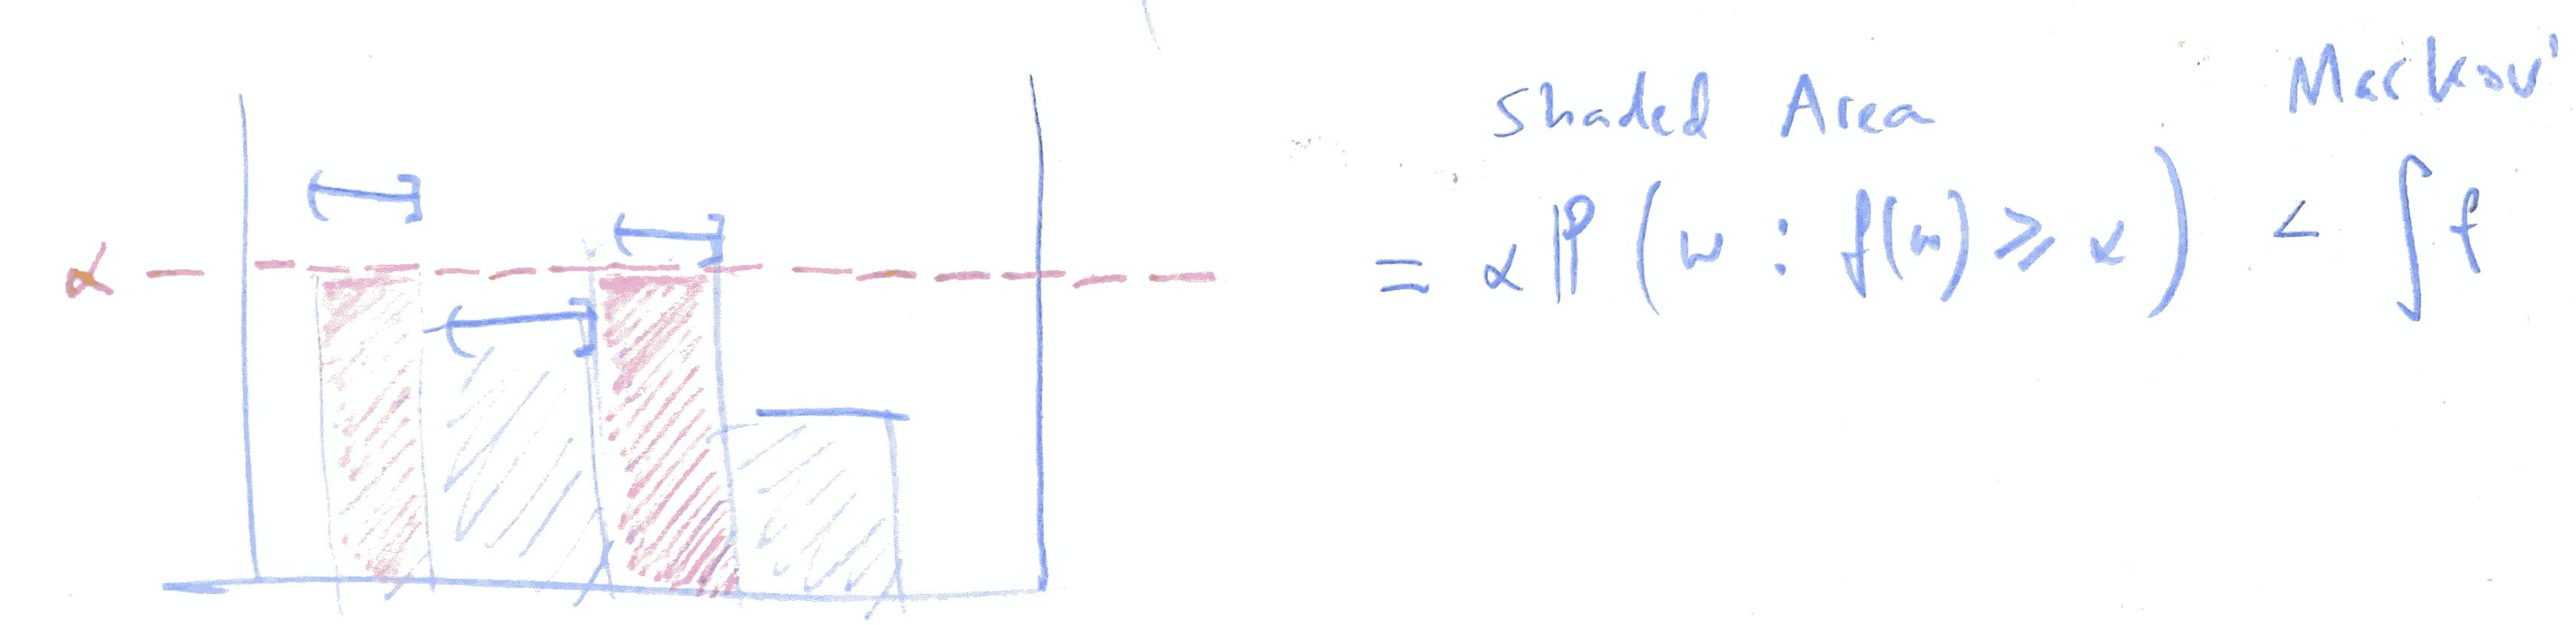
\includegraphics[width=400pt]{img/analysis--real-analysis--measure-theory--weak-law-of-large-numbers-c9c2.png}

  If $X \sim \Unif(0, 1)$ then the RHS is $\E[X]$.

\end{intuition}


\begin{proof}
  [me]

  Clearly
  \begin{align*}
    \int_{f(x) \geq \alpha} f \leq \int_{[0, 1]} f.
  \end{align*}
  Therefore
  \begin{align*}
    \int_{f(x) \geq \alpha} \alpha \leq \int_{[0, 1]} f
  \end{align*},
  or equivalently
\begin{align*}
  \alpha \int \textbf{1}_{f(x) \geq \alpha} \leq \int_{[0, 1]} f,
\end{align*}
which is the same thing as
  \begin{align*}
    \alpha P\Big(\Big\{x: f(x) \geq \alpha\Big\}\Big) < \int_0^1 f(x) \dx.
  \end{align*}
\end{proof}

\begin{theorem}[Weak Law of Large Numbers]
  Fix an $\epsilon > 0$. Then
  \begin{align*}
    \lim_{n \to \infty}P\Big(\Big\{\om: \frac{1}{n}\big|\sum_{i=1}^n r_i(\om)\big| \geq \epsilon\Big\}\Big) = 0.
  \end{align*}
\end{theorem}

In other words: we move through all the $\om \in [0, 1]$. For a given $\om \in [0, 1]$, compare the number
of $0$s and $1$s in the first $n$ digits of the binary expansion, and record the excess as a proportion of $n$;
this is $\frac{1}{n}|s_n(\om)|$. The theorem states that for all $\epsilon > 0$ the probability measure
associated with the set of $\om$s for which $\frac{1}{n}|s_n(\om)| > \epsilon$ goes to $0$ as $n \to \infty$.

\begin{proof}
  Fix an $\epsilon > 0$. We square both sides of the inequality, instead of working with the absolute value. So
  what we want to show is that $P\big(\big\{\om: s_n^2(\om) \geq n^2\epsilon^2\big\}\big) \to 0$
  as $n \to \infty$.

  It would be nice to find an expression for this probability measure as a function of $n$. However, what we'll
  do is find an upper bound: that will suffice also.

  Note that $s_n(\om)$ is a step function (and so $s_n^2(\om)$ is also):

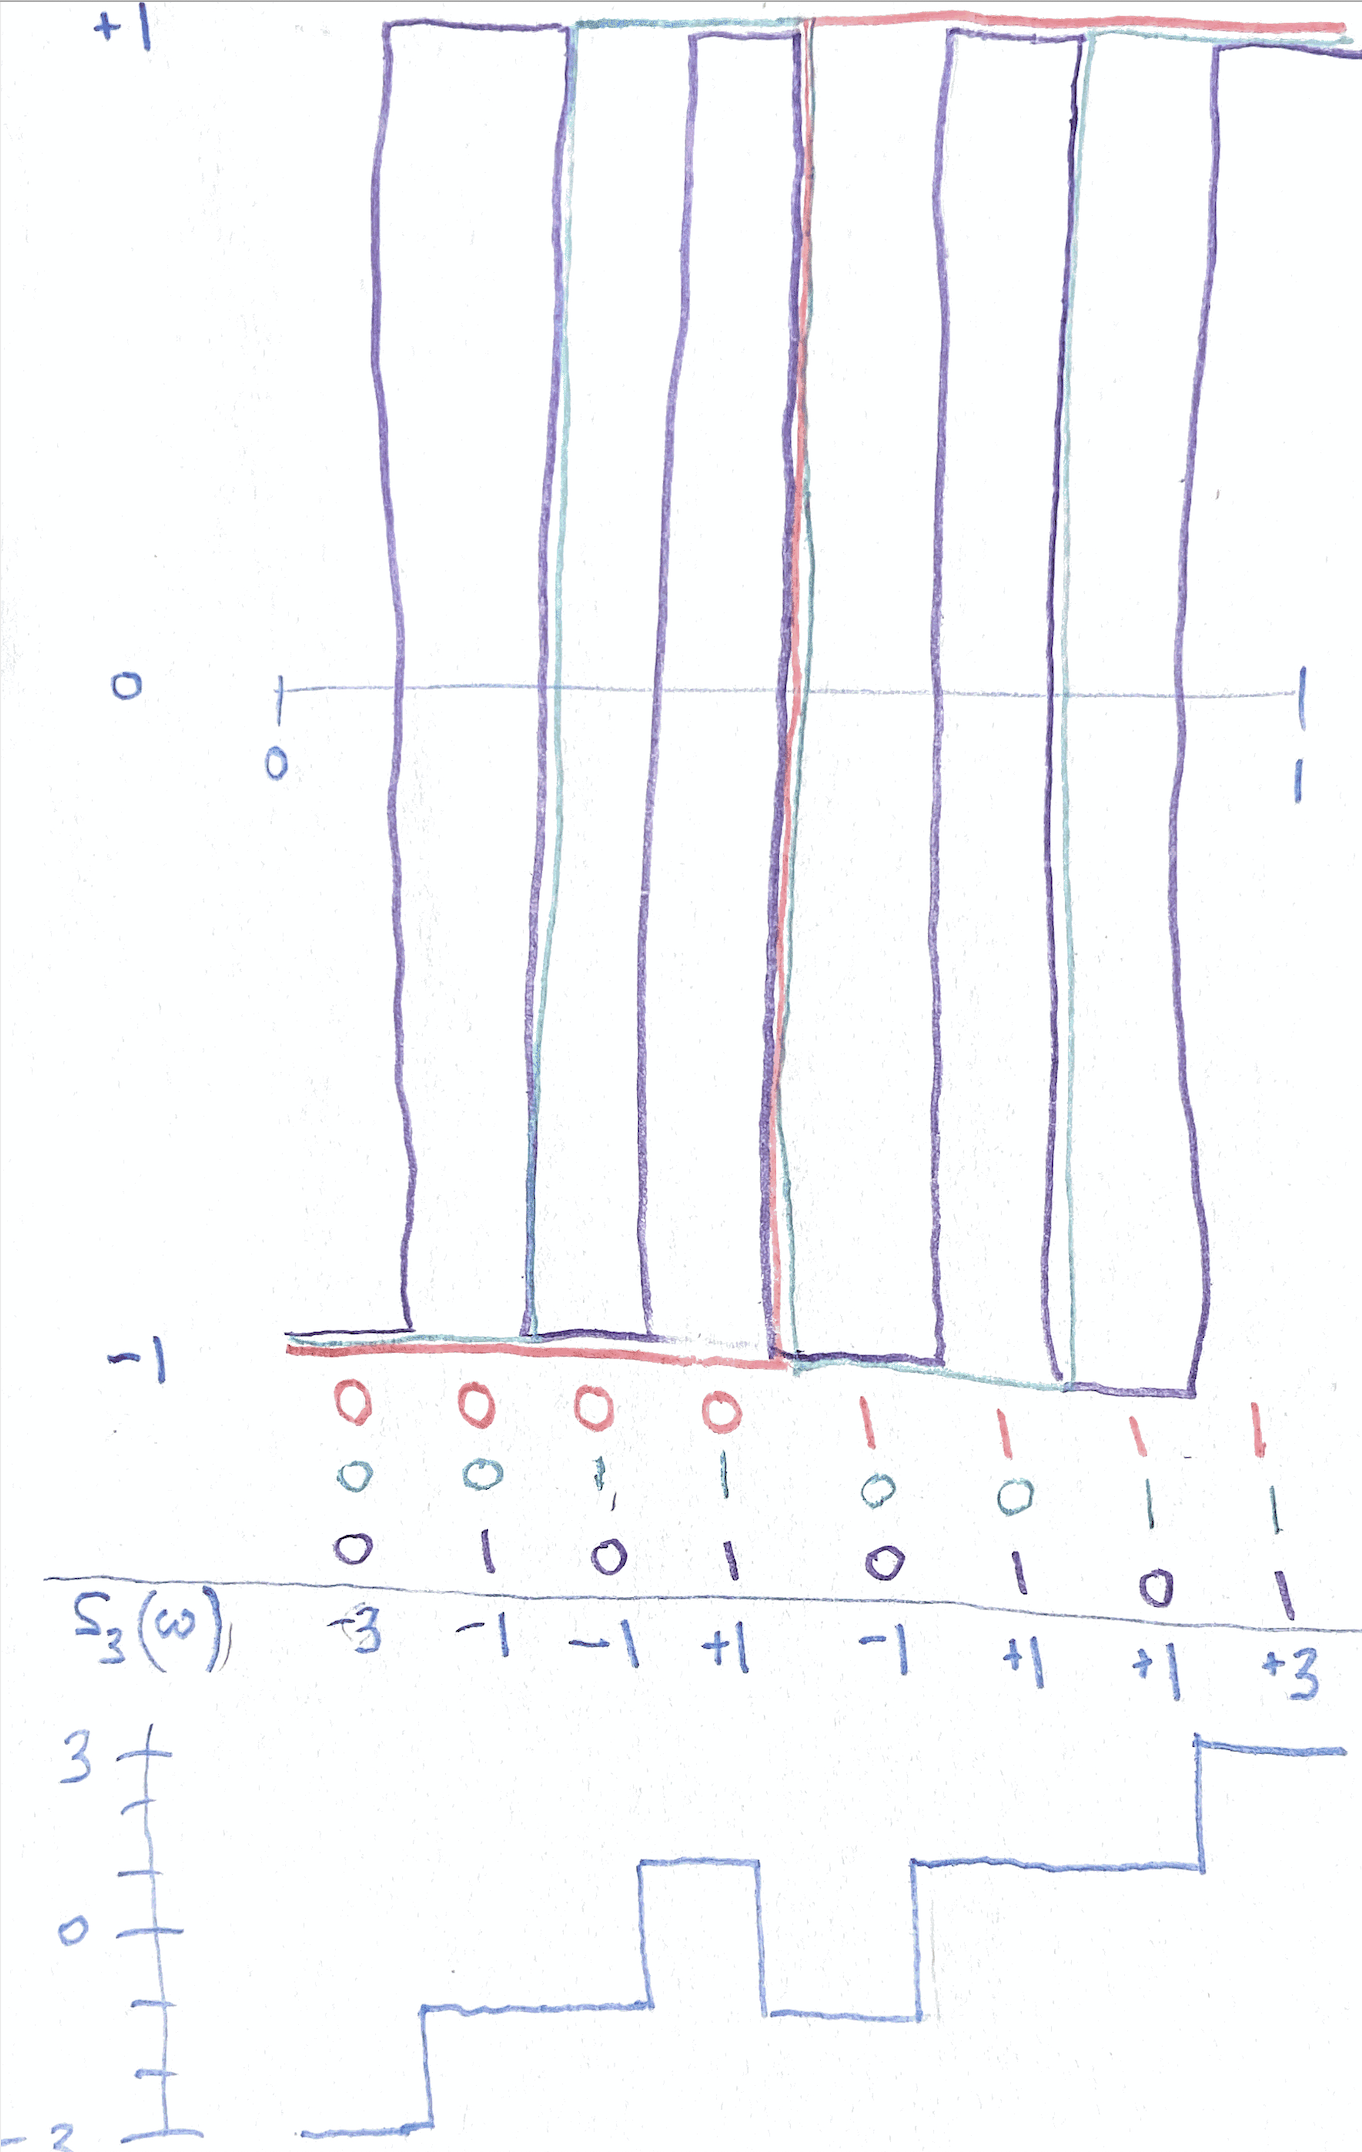
\includegraphics[width=400pt]{img/analysis--real-analysis--measure-theory--weak-law-of-large-numbers-c049.png}


By Markov's inequality / ``Shaded Area lemma​'' we have
\begin{align*}
  n^2\epsilon^2P\Big(\Big\{\om: s_n^2(\om) \geq n^2\epsilon^2\Big\}\Big) \leq \int_0^1 s_n^2(\om) \d\om = n
\end{align*}
and therefore
\begin{align*}
  P\Big(\Big\{\om: s_n^2(\om) \geq n^2\epsilon^2\Big\}\Big) \leq  \frac{1}{n\epsilon^2},
\end{align*}
which proves the desired result since it shows that the probability measure is bounded above by a quantity that
goes to $0$ as $n \to \infty$.
\end{proof}

\subsection{Strong Law of Large Numbers}

\begin{definition}[negligible, null set]
  A set $A$ is \defn{negligible} if, for any $\epsilon > 0$, it can be covered by a finite or countable
  union $\bigcup_k I_k$ of intervals with $\sum_k |I_k| < \epsilon$.
\end{definition}

Recall the weak law of large numbers:
  \begin{align*}
    \lim_{n \to \infty}P\Big(\Big\{\om: \frac{1}{n}\big|s_n(\om)\big| \geq \epsilon\Big\}\Big) = 0.
  \end{align*}

\begin{definition}[Normal numbers]
  Define the set of \defn{normal numbers} to be
  \begin{align*}
    N = \Big\{\om ~:~ \lim_{n\to\infty} \frac{1}{n}s_n(\om) = 0 \Big\}.
  \end{align*}
\end{definition}

\begin{theorem*}[Borel's normal number theorem]
  $N^c = \R \setminus N$ is negligible.
\end{theorem*}

\begin{intuition}
  Visualize the $s_n$ sequence of a non-normal number $\om$, stretching off to infinity. However far we’ve
  gone, there will always be another point further along at which an excursion of the random walk sticks out
  further than $\eps$. But despite the fact that this must always happen, it’s less and less likely the further
  we go. tThe fact that it must always happen again corresponds to the fact that we can write the event as a
  countable union: (happened by this generation) union with (happened at the next generation), etc. But at the
  same time, since it’s getting harder and harder, for any given $\gamma >0$ we can find some generation $m$
  beyond which the union sums to less than $\gamma$. nevertheless , the event is equal to the union beyond that
  point, since the departures must always keep occurring (otherwise the number would be normal). So the union
  doesn’t have to include earlier generations.

  This is why the complement of the normal numbers is negligible. Perhaps it’s typical of negligible sets that
  they correspond to an event that must always occur one more time, and yet get ever less and less likely?
\end{intuition}

\begin{proof}
  Recall that we are trying to find an ``efficent covering​'' of $N^c$.

  Let $(\eps_n)$ be a sequence that converges to zero, and define a sequence of sets $(A_n)$,
  where
  \begin{align*}
    A_n = \Big\{\om : \Big|\frac{1}{n} s_n(\om)\Big| \geq \eps_n\Big\}.
  \end{align*}
  (We can think of $A_n$ as the set of $\om$ whose binary expansions are ``not normal so far​''.)

  Note that, for any given $m$, we have the following: a number that stays inside $\eps_n$ for ever is normal:
  \begin{align*}
    \Big(\bigcap_{n=m}^\infty A_n^c\Big) \subset N.
  \end{align*}
  Equivalently, a non-normal number must stray outside $\eps_n$ at some point:
  \begin{align*}
    N^c \subset \Big(\bigcup_{n=m}^\infty A_n\Big).
  \end{align*}
  Recall that our aim is to cover $N^c$ with a countable union of intervals, where the total length of the
  intervals is arbitrarily small: if we can show that the $A_n$ meet that description then we are done.

  Note that each set $A_n$ is a finite disjoint union $\bigcup_{k}I_{nk}$ of intervals
  with $P(A_n) = \sum_k |I_{nk}|$. So what we need to do is show that, for any given $\gamma > 0$, there exists
  a sequence $(\eps_n)$ converging to zero, and an $m$, such that $\sum_{n=m}^\infty P(A_n) < \gamma$.

  At this point, we need to find an expression for an upper bound on $P(A_n)$ in terms of $n$ and $\eps_n$.
  From the lemma, we have
  \begin{align*}
    P(A_n) \leq \frac{3}{n^2\eps_n^4},
  \end{align*}
  so we would like to find $(\eps_n)$ and $m$ such that
  \begin{align*}
    \sum_{n=m}^\infty \frac{3}{n^2\eps_n^4} < \gamma.
  \end{align*}
  To do so, we need only choose $(\eps_n)$ so that the series $\sum_nn^{-2}\eps_n^{-4}$
  converges: $\eps_n = n^{-1/8}$ will do. Then, since the series converges, there exists an $m$ such that the
  tail sums to less than $\gamma$, as required.
\end{proof}

\begin{lemma}
  For all $n \in \N$, we have (from Markov's inequality)
  \begin{align*}
    P\Big(\Big\{ \om : |s_n(\om)| \geq n\eps  \Big\}\Big) \leq \frac{1}{n^4\eps^4} \int_0^1 s_n^4(\om) \d\om,
  \end{align*}
  and (by considering integrals of products of four Rademacher functions)
  \begin{align*}
    \int_0^1 s_n^4(\om) \d\om \leq 3n^2.
  \end{align*}
  Therefore
  \begin{align*}
    P\Big(\Big\{ \om : \frac{1}{n}\big|s_n(\om)\big| \geq \eps  \Big\}\Big) \leq \frac{3}{n^2\eps^4}.
  \end{align*}
\end{lemma}